\documentclass[12pt, a4paper]{article}

% ── Packages ──────────────────────────────────────────────────────────────────
\usepackage[utf8]{inputenc}
\usepackage[T1]{fontenc}
\usepackage{geometry}
\geometry{margin=2.5cm}
\usepackage{authblk}
\usepackage{hyperref}
\usepackage{url}
\usepackage{natbib}
\usepackage{setspace}
\usepackage{titlesec}
\usepackage{booktabs}
\usepackage{graphicx}
\usepackage{amsmath}
\usepackage{lineno}
\linenumbers
\doublespacing

% ── Running head (manual) ─────────────────────────────────────────────────────
\usepackage{fancyhdr}
\setlength{\headheight}{14pt}
\pagestyle{fancy}
\fancyhf{}
\lhead{\small Geomorphological Connectivity and Temporal Controls}
\rhead{\small M. Muzzamil et al.}
\cfoot{\thepage}

% ── Helper commands to replace Copernicus-specific macros ─────────────────────
\newcommand{\runningtitle}[1]{}
\newcommand{\runningauthor}[1]{}
\newcommand{\correspondence}[1]{\footnote{Correspondence: #1}}
\newcommand{\received}[1]{}
\newcommand{\pubdiscuss}[1]{}
\newcommand{\accepted}[1]{}
\newcommand{\published}[1]{}
\newcommand{\firstpage}[1]{}

% Section-level wrappers for Copernicus back-matter macros
\newcommand{\codeavailability}{\section*{Code availability}}
\newcommand{\dataavailability}{\section*{Data availability}}
\newcommand{\authorcontribution}{\section*{Author contributions}}
\newcommand{\competinginterests}{\section*{Competing interests}}
\newcommand{\acknowledgements}{\section*{Acknowledgements}}

% Copernicus uses \introduction instead of \section{Introduction}
\newcommand{\introduction}{\section{Introduction}}

% ── Helper commands to replace Elsevier-specific macros ───────────────────────
\usepackage{keyval}
\makeatletter
\providecommand{\ead}[1]{\footnote{Email: \href{mailto:#1}{\texttt{\detokenize{#1}}}}}
\providecommand{\corref}[1]{$^*$}
\providecommand{\cortext}[2][]{}
\define@key{aff}{organization}{\def\aff@org{#1}}
\define@key{aff}{addressline}{\def\aff@addr{#1}}
\define@key{aff}{city}{\def\aff@city{#1}}
\define@key{aff}{postcode}{\def\aff@post{#1}}
\define@key{aff}{country}{\def\aff@country{#1}}
\providecommand{\affiliation}[2][]{%
  \def\aff@org{}%
  \def\aff@addr{}%
  \def\aff@city{}%
  \def\aff@post{}%
  \def\aff@country{}%
  \setkeys{aff}{#2}%
  \affil[#1]{%
    \ifx\aff@org\@empty\else\aff@org\fi
    \ifx\aff@addr\@empty\else, \aff@addr\fi
    \ifx\aff@city\@empty\else, \aff@city\fi
    \ifx\aff@post\@empty\else--\aff@post\fi
    \ifx\aff@country\@empty\else, \aff@country\fi
  }%
}
\makeatother

% ── Document ──────────────────────────────────────────────────────────────────
\begin{document}

\title{\textbf{Geomorphological Connectivity and Temporal Hydrological Controls\\
of Surface Water Dynamics in the Indus River Delta}}

\author[inst1]{Mirza Muhammad Muzzamil\corref{cor1}}
\ead{mirzamuzzamil@neduet.edu.pk}

\author[inst1]{Muhammad Ali Ismael}
\ead{maismael@neduet.edu.pk}

\author[inst2]{Syed Imran Ahmad}
\ead{imranahmad@neduet.edu.pk}

\author[inst3]{Rustam B. Rustomov}
\ead{r_rustomov@hotmail.com}

\cortext[cor1]{Corresponding author.}

\affiliation[inst1]{
    organization={Department of Computer and Information Systems Engineering (CISE), NED University of Engineering and Technology},
    addressline={University Road},
    city={Karachi},
    postcode={75270},
    country={Pakistan}
}

\affiliation[inst2]{
    organization={Department of Civil Engineering, NED University of Engineering and Technology},
    addressline={University Road},
    city={Karachi},
    postcode={75270},
    country={Pakistan}
}

\affiliation[inst3]{
    organization={Department of Scientific Innovations and External Relations, Institute of Physics, Ministry of Science and Education of the Republic of Azerbaijan},
    addressline={33 H. Javid Avenue},
    city={Baku},
    postcode={AZ1143},
    country={Azerbaijan}
}

\date{}
\maketitle

\thispagestyle{fancy}

% ── Abstract ──────────────────────────────────────────────────────────────────
\begin{abstract}
Mapping high-resolution surface water in dynamic deltas is critical for water resource management. Most empirical machine-learning approaches map spectral reflectances directly to water masks, bypassing physical catchment state representations. We evaluate geomorphological and temporal controls on surface water in the Indus River Delta (Pakistan) from 2018 to 2024. Using 83,000 monthly GEE records, we analyze Random Forests, LSTMs, and Transformers under a leakage-free input configuration. Sequence models exhibited collapse under the evaluated coordinate-withheld setting during dry periods ($F_1\text{-score} = 0.000$) due to scale mismatches between coarse climate forcings and sub-pixel channels. During extreme floods, spatial Random Forests outperform sequence models ($F_1\text{-score} = 0.845$ vs. $0.745$) because static features constrain water boundaries. Ablation experiments show that a Terrain-only model achieves an $F_1\text{-score}$ of 0.842 (95\% CI: [0.833, 0.851]), which shows no statistically significant difference from the Combined model ($F_1\text{-score} = 0.845$; McNemar's $p = 0.2584$, representing limited statistical power to detect small differences rather than proof of equivalence). These results indicate that high-resolution geomorphological constraints explain the spatial organization of inundation boundaries under the evaluated feature set, whereas coarse meteorological forcing primarily regulates temporal activation. Furthermore, lag correlation audits identify a 3-month upstream precipitation routing delay in coastal wetlands and evaluate a negative correlation in croplands ($r = -0.299$) that remains ambiguous due to confounding crop phenology and irrigation signals. These findings motivate the future development of physically constrained hydrological state-space models.

\end{abstract}

% ── Main body ─────────────────────────────────────────────────────────────────
\introduction
% Section heading emitted by \introduction in main.tex
High-resolution satellite mapping of surface water is key for disaster management and coastal conservation \citep{Wu2020Ensemble}. High-resolution datasets like the Joint Research Centre (JRC) Global Surface Water product highlight rapid changes in terrestrial hydrology under climate change and human regulation \citep{Pekel2016Highresolution}. Recent advances leverage deep neural networks to segment surface water from active microwave or optical imagery \citep{Bazi2021Vision, Phan2020Land}. 

However, these empirical models operate as static spatial mappings. They bypass intermediate land surface states (e.g., storage or soil saturation) and ignore temporal catchment memory \citep{Nearing2020What}. In coastal deltas, this is highly problematic because upstream reservoir regulation and canal irrigation networks introduce non-linear anthropogenic lags that decouple local precipitation from local wetness, leading to spatial overfitting and temporal representation collapse.

Although previous research has successfully applied remote sensing classifiers and deep learning to map deltaic inundation, many existing frameworks treat geomorphological constraints and meteorological drivers as joint statistical features. They frequently fail to separate their individual predictive weights or identify the boundaries where topographic controls and climate triggers decouple. Consequently, previous models are insufficient because combining these features masks spatial extrapolation errors in new basins and leads to representation collapse during dry seasons when coarse climate data cannot resolve sub-grid channel networks. This study is scientifically necessary to isolate these controls under a coordinate-withheld, leakage-free design, establishing where meteorological inputs may fail to resolve fine topographic structures. This study provides a rigorous, spatially independent benchmark for separating geomorphological and meteorological controls on surface water dynamics in a highly regulated deltaic basin. By doing so, we position our work against traditional empirical classifiers by highlighting the physical limits of data-driven models under spatial and temporal scale mismatches.

Unlike previous delta flooding studies that treat geomorphological and meteorological variables as joint predictors, this work separates their roles using a leakage-free design, a point-level spatial split, and residual spatial autocorrelation testing. This allows us to quantify where static terrain explains spatial flood boundaries and where coarse climate forcing may fail to resolve sub-pixel hydrological structure.

To achieve these objectives, we present five primary scientific contributions, each directly supported by our experimental design and statistical audits. First, we establish a leakage-free flood prediction benchmark that excludes concurrent satellite observations, ensuring that the models rely solely on static terrain and antecedent climate features. Second, we execute a terrain-meteorological feature ablation study: Terrain features account for 87.81\% of the Random Forest Gini feature importance, representing model-specific predictive weights rather than direct physical causality. Concurrently, we find that Terrain-only and Combined models are statistically indistinguishable, with overlapping bootstrap confidence intervals. Third, we characterize temporal routing lag and irrigation decoupling, identifying a multi-month routing delay in coastal wetlands and an out-of-phase divergence in croplands. Fourth, we perform a spatial autocorrelation residual audit, showing that Moran's I on validation residuals is statistically indistinguishable from zero, which suggests that our disjoint coordinate split successfully prevented spatial leakage. Fifth, we diagnose sequence model representation collapse, showing that LSTMs and Transformers default to dry-class predictions when spatial coordinates are withheld, highlighting a resolution mismatch. These results indicate that high-resolution geomorphological constraints explain the spatial organization of inundation boundaries under the evaluated feature set, whereas coarse meteorological forcing primarily regulates temporal activation.


\section{Literature Review}

\subsection{Remote Sensing and Surface Water Mapping}
Surface water mapping has progressed from optical index thresholding \citep{Amani2020Google} to high-resolution global products like the 30-meter Joint Research Centre (JRC) Global Surface Water dataset \citep{Pekel2016Highresolution, Liu2021FinerResolution, Yang202130}. Because cloud cover restricts optical sensors, active microwave Synthetic Aperture Radar (SAR) is widely used for all-weather flood delineation \citep{Twele2016Sentinel1}. Machine learning models, such as Random Forests and Vision Transformers, segment these radar backscatter signals to map complex boundaries \citep{Phan2020Land, Bazi2021Vision}.

However, these classifiers operate as static spatial mappings without representing temporal catchment memory or mass conservation. We address this by employing a leakage-free configuration that excludes concurrent satellite observations, forcing models to predict surface water dynamics using only static geomorphology and antecedent meteorological forcing to isolate their relative contributions.

\subsection{Machine Learning and Sequence Modeling in Hydrology}
Data-driven models, particularly Long Short-Term Memory (LSTM) networks, excel in rainfall-runoff modeling by capturing temporal catchment memory from meteorological sequences \citep{Kratzert2018, Sit2020A, Wünsch2021Groundwater}. Recurrent neural networks can also ingest static catchment attributes to regionalize predictions across ungauged basins \citep{Kratzert2019}. Recently, attention-based Transformers have scaled predictions globally \citep{Nearing2024Global, Feng2023The}.

However, these sequence models typically focus on lumped outlet discharge and rely on coarse meteorological inputs (5 to 9\,km) that cannot resolve sub-pixel channels. When spatial coordinates are withheld to isolate temporal climate-driven dynamics, empirical sequence models suffer from representation collapse. We address this by evaluating LSTMs and Transformers on a point-level dataset to characterize this scale mismatch under a coordinate-withheld configuration.

\subsection{Physics-Informed Neural Networks and Differentiable Hydrology}
To prevent empirical models from violating conservation laws, physics-informed machine learning (PIML) integrates mass-balance constraints and differentiable process models with neural networks \citep{Karniadakis2021Physicsinformed, Shen2023Differentiable}. Differentiable models parameterize physical routing schemes (e.g., the HBV model), enabling predictions that respect mass conservation \citep{Feng2023The, Zhao2022Evaporative, Li2020Toward}. However, these approaches focus on catchment-scale outlet discharge rather than high-resolution spatial mapping. We address this limit by motivating the future development of physically constrained state-space models that conceptually integrate temporal mass balance with spatial geomorphological constraints.

\subsection{Delta Hydrology and Catchment Memory}
Coastal river deltas are complex environments governed by interacting upstream discharge, tides, precipitation, and canal withdrawals \citep{Wu2020Ensemble}. Upstream runoff can take months to route through reservoirs and barrages, decoupling local rainfall from deltaic flooding \citep{Scanlon2023Global, Lall2020A}. This routing delay is further modified by groundwater dynamics and vegetation water storage \citep{Jiao2021Observed, Dorigo2021The, Poggio2021SoilGrids} under changing climate regimes \citep{Tabari2020Climate, Berdugo2020Global, Jasechko2024Rapid, Gleeson2020Global, Lian2020Summer, MuñozSabater2021ERA5Land, Funk2015The}. In the Indus Delta, natural hydrology is heavily altered by massive upstream canal systems and barrages built since the 1960s \citep{Giosan2006Recent, Syvitski2009Sinking, Dunn2019Projections, Solangi2019Analysis, Salik2022Social}. Deltaic hydrodynamics are governed by upstream river discharge \citep{Karim2002Water}, local irrigation diversions \citep{Cheema2012Surface}, and tidal ocean pressure \citep{Salik2016Environmental, Mitra2024Assessing}, routed through complex channel networks \citep{Tejedor2015Delta1, Tejedor2015Delta2}.

However, prior deltaic studies treat geomorphology and climate forcing as joint statistical predictors without isolating their relative weights. Furthermore, the role of canal irrigation in decoupling rainfall-wetness relationships remains poorly integrated into machine learning studies. We address these limitations by executing Global Moran's I and cross-correlation lag audits to identify a 3-month routing delay in coastal wetlands and evaluate a negative precipitation-wetness correlation in croplands ($r = -0.299$), characterizing the decoupling boundary where local rainfall and human water management intersect.
Collectively, previous studies demonstrate significant progress in remote sensing flood mapping, sequence modelling, and differentiable hydrology. However, few studies have explicitly separated geomorphological constraints from meteorological forcing under leakage-controlled conditions.

\begin{table*}[t]
\caption{Literature review matrix summarizing objectives, methods, and limitations of key studies in remote sensing flood mapping and hydrological AI.}
\label{tab:literature_review}
\centering
\footnotesize
\resizebox{\textwidth}{!}{%
\begin{tabular}{p{2.0cm} c p{2.5cm} p{3.0cm} p{2.8cm} p{4.0cm}}
\hline
\textbf{Author} & \textbf{Year} & \textbf{Journal} & \textbf{Objective} & \textbf{Method} & \textbf{Limitation} \\
\hline
Pekel et al. & 2016 & Nature & Global surface water occurrence mapping & Random Forest classification of Landsat series & Vulnerable to cloud occlusion; neglects temporal catchment memory \\
Twele et al. & 2016 & NHESS & Automated Sentinel-1 flood mapping & Split-based thresholding and fuzzy logic & Relies on concurrent SAR overpasses; ignores temporal climate memory \\
Kratzert et al. & 2018 & HESS & Rainfall--runoff streamflow prediction & Long Short-Term Memory (LSTM) network & Operates on lumped basin discharge; cannot map 2D inundation boundaries \\
Kratzert et al. & 2019 & HESS & Regionalization in ungauged basins & Entity-Aware LSTM (EA-LSTM) with static features & Focuses on lumped discharge points; ignores spatial routing networks \\
Wu et al. & 2020 & WIRES Water & Overview of flood forecasting & Ensemble numerical weather and hydrologic models & Neglects sub-pixel spatial boundaries and local geomorphology \\
Nearing et al. & 2020 & WRR & Assessment of ML in streamflow forecasting & LSTM neural network compared to process models & Lacks spatial context; cannot map flood boundaries \\
Tejedor et al. & 2015 & WRR & Delta network connectivity and topology & Graph-theoretic transport and vulnerability metrics & Focuses on network geometry; does not integrate dynamic climate triggers \\
Muñoz-Sabater et al. & 2021 & ESSD & Global high-resolution reanalysis dataset & ERA5-Land reanalysis model integration & Coarse resolution (9 km) fails to resolve sub-pixel channels \\
Feng et al. & 2023 & HESS & Physics-informed hydrologic modeling & Process-based differentiable modeling & High computational cost; parameter equifinality in ungauged areas \\
\hline
\end{tabular}%
}
\end{table*}



\section{Study Area}
The study is conducted in the \textbf{Indus River Delta} (Fig.~\ref{fig:study_area}), located in the southern part of Sindh Province, Pakistan ($23.0^\circ\text{N}$ to $24.8^\circ\text{N}$, $67.0^\circ\text{E}$ to $69.0^\circ\text{E}$). The Indus Delta is a highly dynamic and ecologically vulnerable coastal wetland system, covering an area of approximately $30,000~\text{km}^2$. It is characterized by an arid to semi-arid climate, receiving less than $250~\text{mm}$ of annual rainfall, which occurs almost entirely during the summer monsoon (July--September).

\begin{figure}[t]
\centering
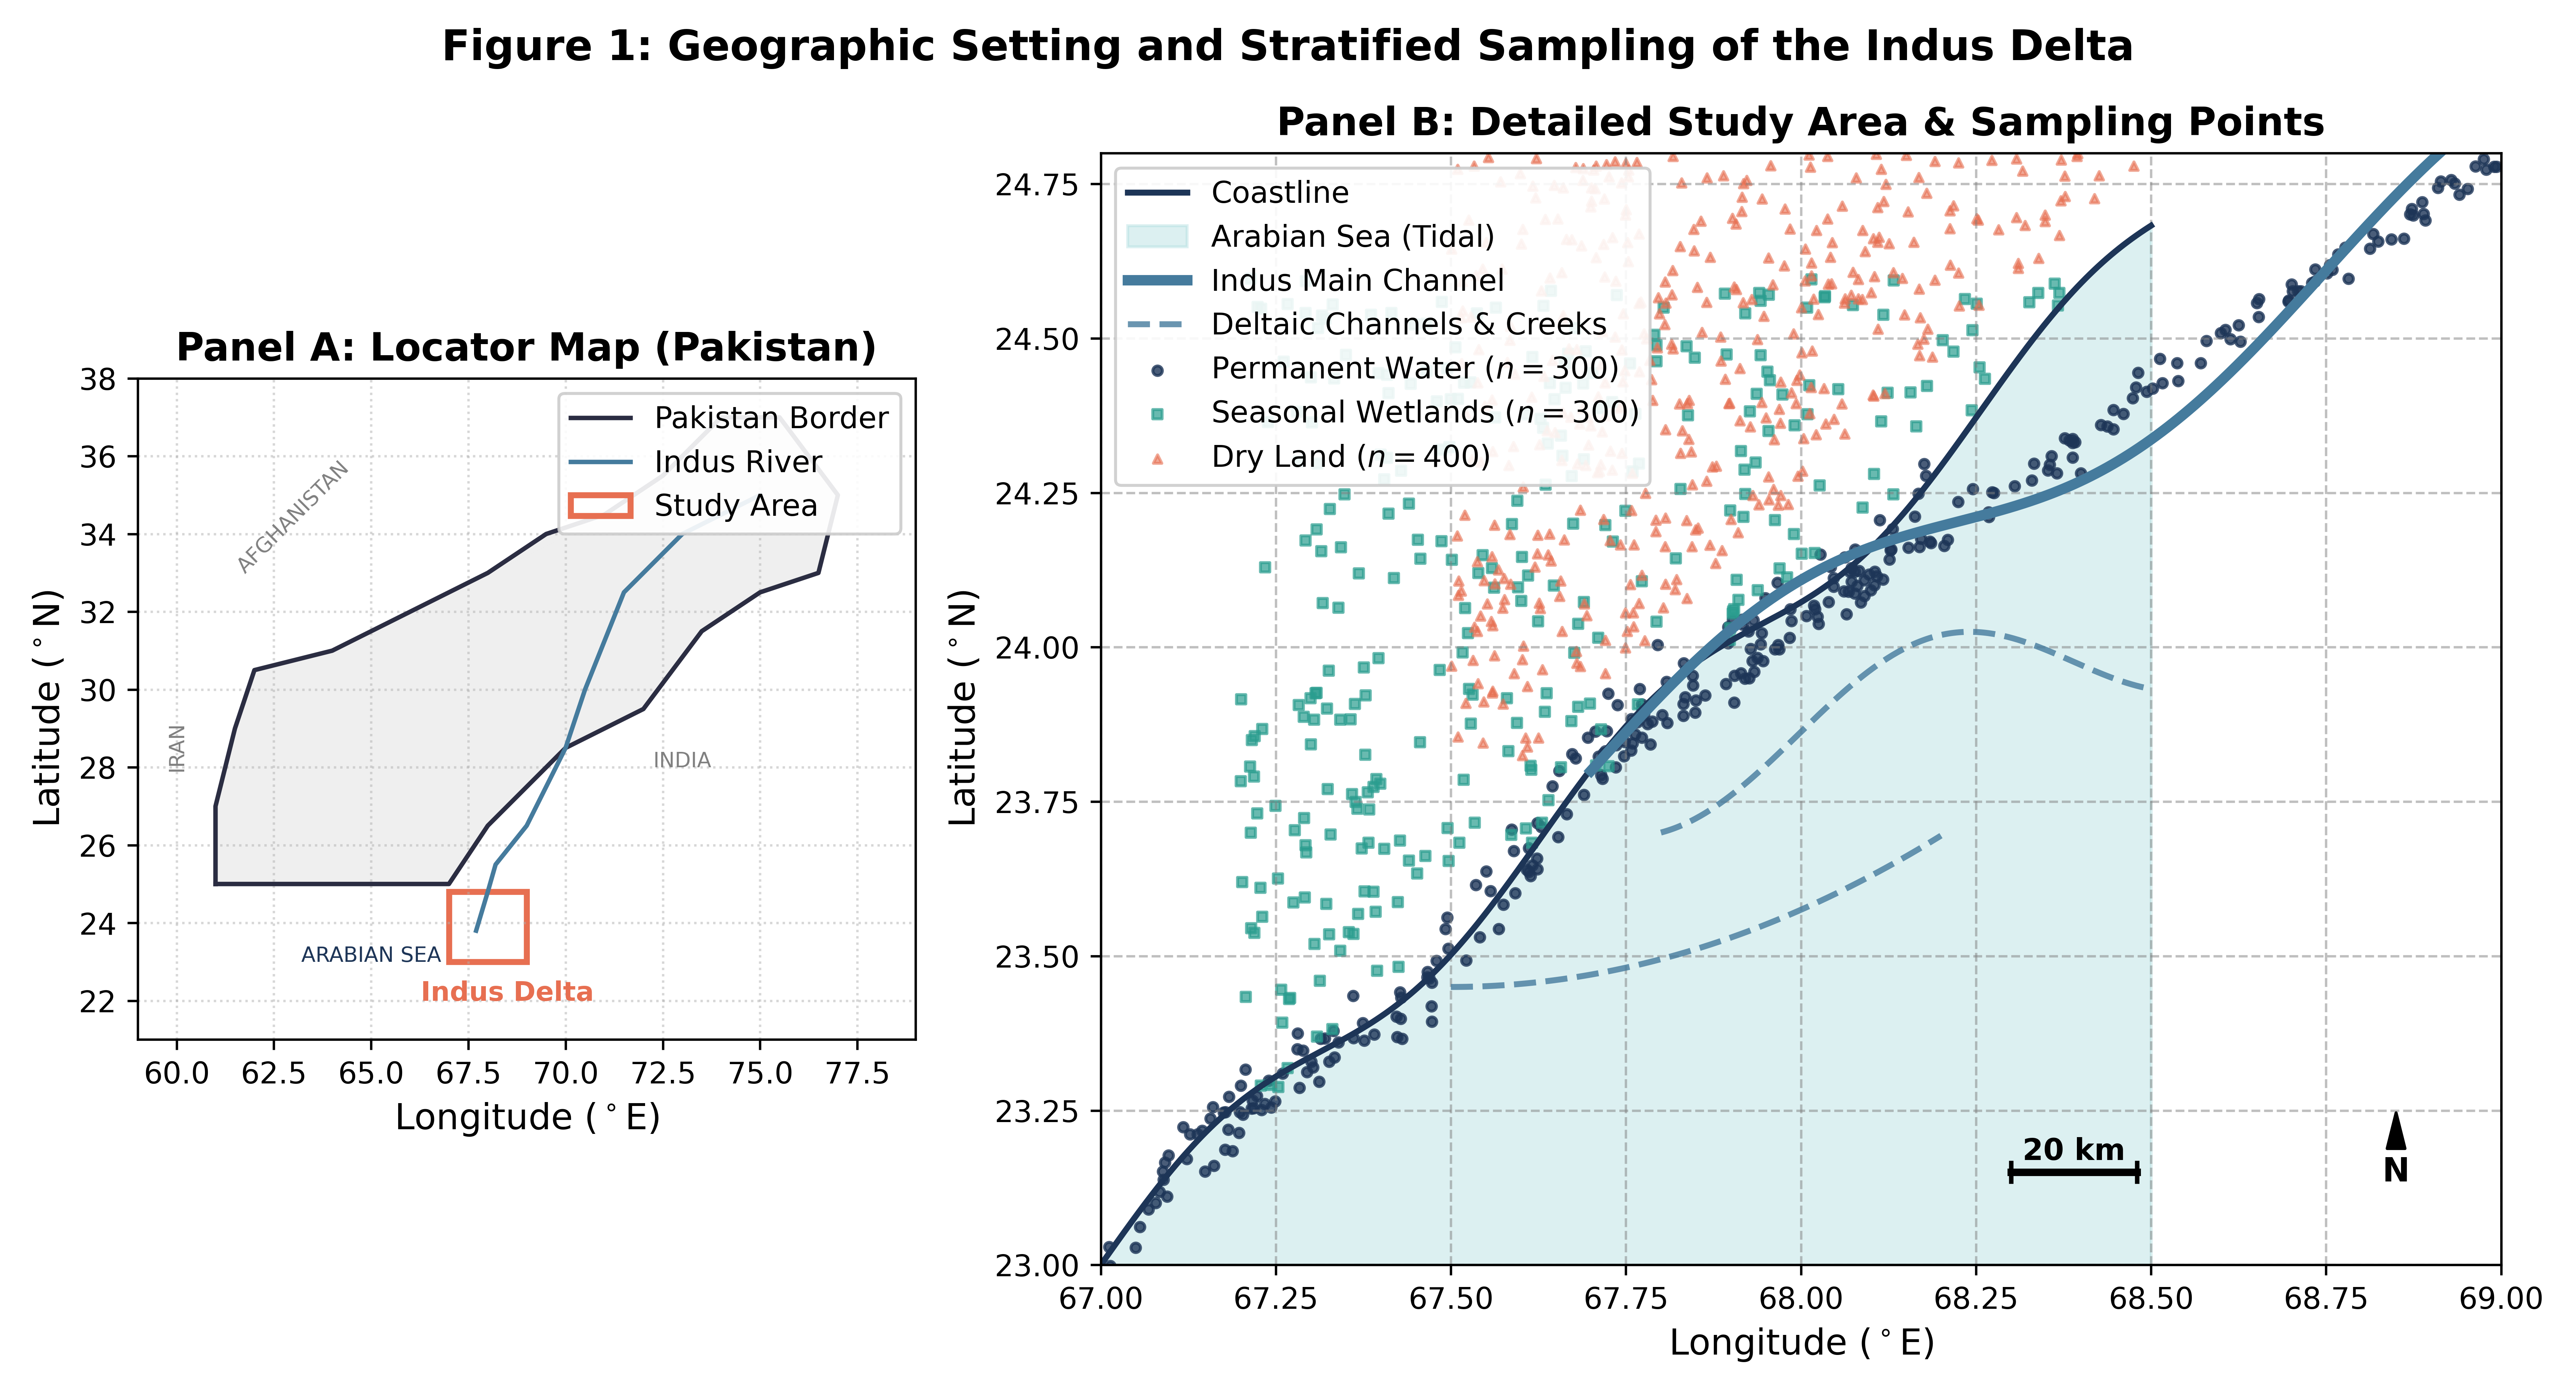
\includegraphics[width=0.95\linewidth]{figures/fig1_study_area.png}
\caption{Geographic setting and stratified point sampling design of the Indus River Delta. Panel A shows the locator map of Pakistan with the Indus River routing and the study area footprint. Panel B shows the detailed zoom-in of the delta, illustrating the coastline, main river channels, tidal creeks, and the distribution of the $1,000$ stratified random sampling points (permanent water, seasonal wetlands, and dry land) derived from historical JRC surface water occurrence.}
\label{fig:study_area}
\end{figure}

The deltaic hydrology is dominated by three main drivers:
\begin{enumerate}
    \item \textbf{Monsoonal Upstream Discharge:} The Indus River routes discharge from the Upper Indus Basin (meltwater from Hindu Kush-Karakoram-Himalayan glaciers and monsoon rainfall). This discharge is heavily regulated upstream by the Tarbela and Mangla reservoirs and a series of barrages. Historically, the river delivered a mean annual inflow of approximately $150~\text{billion cubic meters (BCM)}$ to the delta. However, extensive upstream diversions at the Kotri Barrage—the final downstream control structure—have reduced this to less than $10~\text{BCM}$ in normal years, though peak monsoonal floods (such as in 2022) can exceed $15,000~\text{m}^3~\text{s}^{-1}$.
    \item \textbf{Canal Irrigation Network:} A dense network of canals supplies freshwater to agricultural fields in the delta. The canal command area in the delta covers approximately $1~\text{million hectares}$, representing a highly managed sub-catchment where withdrawals redirect substantial freshwater volumes, creating localized surface water dynamics that are completely decoupled from local meteorological precipitation.
    \item \textbf{Coastal Tidal Inundation:} The delta's coastline is intersected by numerous creeks and mangrove wetlands subject to semi-diurnal tides with a mean tidal range of $2.0$ to $3.5~\text{m}$ at the coast. Seawater intrusion routes tidal head changes up to $80~\text{km}$ inland through topological pathways, affecting soil salinity and moisture persistence.
\end{enumerate}

During extreme meteorological anomalies (such as the historical 2022 Pakistan monsoon floods), river discharge exceeds barrage capacities, causing widespread inundation across the delta. In contrast, during normal dry seasons, active flow is confined to main channels and tidal creeks, while agricultural fields experience drydowns.


\section{Datasets}
To analyze surface water dynamics, we compiled a high-resolution spatial-temporal dataset over the Indus Delta spanning the years 2018 to 2024. The dataset consists of 1,000 spatial point locations sampled across the delta, yielding a total of 83,000 monthly records over 83 sequential months (excluding August 2018 due to 100\% cloud cover).

\subsection{Stratified Sampling Design}
To capture the full spectrum of hydrological conditions, the 1,000 point locations were selected using a stratified random sampling design based on the long-term JRC Global Surface Water occurrence dataset \citep{Pekel2016Highresolution}:
\begin{itemize}
    \item \textbf{Permanent Water (300 points):} Selected from areas with a historical water occurrence probability $> 50\%$, corresponding to main river channels, active creeks, and deep lakes.
    \item \textbf{Seasonal Wetlands (300 points):} Selected from areas with water occurrence probabilities between $1\%$ and $50\%$, representing floodplains, agricultural marshes, and tidal mudflats.
    \item \textbf{Dry Land (400 points):} Selected from areas with a historical water occurrence probability of $0\%$, representing arid shrublands, dunes, and urban regions.
\end{itemize}

While this stratified sampling design guarantees that the calibration data contains representation across all land cover categories, it does not alter the intrinsic temporal class imbalance of the system. During normal dry periods (which constitute the vast majority of the time series), the actual surface water occurrence rate among the 1,000 points drops to $8.27\%$. This creates a strong temporal class imbalance that represents a significant challenge for purely empirical sequential classifiers.

\subsection{Google Earth Engine Data Compilation}
At each point location, we extracted monthly aggregated time-series data using Google Earth Engine \citep{Amani2020Google} (data accessed in June 2026). We fetched static terrain features and dynamic meteorological/backscatter bands from the following specific GEE collections:
\begin{itemize}
    \item \textbf{Active Microwave (Sentinel-1 Synthetic Aperture Radar, SAR):} We compiled Interferometric Wide (IW) Ground Range Detected (GRD) products (GEE Asset: \verb|COPERNICUS/S1_GRD|) at $10$~m resolution, extracting vertical-vertical (VV) and vertical-horizontal (VH) polarization bands, as well as the VH/VV ratio. 
    \item \textbf{Multispectral (Sentinel-2 MultiSpectral Instrument, MSI):} We extracted Sentinel-2 surface reflectance products (GEE Asset: \verb|COPERNICUS/S2_SR_HARMONIZED|), calculating five spectral water and vegetation indices: Normalized Difference Vegetation Index (NDVI), Normalized Difference Water Index (NDWI), Modified Normalized Difference Water Index (MNDWI), Land Surface Water Index (LSWI), and Enhanced Vegetation Index (EVI). Cloud masking was applied using the QA60 band, and months with complete cloud cover were omitted.
    \item \textbf{Topography (SRTM $30$~m):} We compiled Shuttle Radar Topography Mission (SRTM) GL1 digital elevation model (DEM) features (GEE Asset: \verb|USGS/SRTMGL1_003|), including elevation, slope, and flow accumulation. We also calculated spatial Euclidean distance to the nearest river channel ($D_{\text{river}}$) and distance to the coastline ($D_{\text{coast}}$).
    \item \textbf{Climate Forcing:} Climate Hazards Group InfraRed Precipitation with Station data (CHIRPS) daily precipitation data (GEE Asset: \verb|UCSB-CHG/CHIRPS/DAILY|) were summed monthly at $0.05^\circ$ resolution \citep{Funk2015The}. Temperature, total evaporation ($ET$), and potential evapotranspiration ($PET$) were compiled from the European Centre for Medium-Range Weather Forecasts (ECMWF) ERA5-Land monthly reanalysis dataset (GEE Asset: \verb|ECMWF/ERA5_LAND/MONTHLY_AGGR|) at $9$~km resolution \citep{MuñozSabater2021ERA5Land}.
\end{itemize}

\subsection{Ground Truth Labeling and Validation}
The binary ground truth occurrence of surface water ($y_i(t) \in \{0, 1\}$) was derived using an established radar backscatter threshold:
\begin{equation}
    y_i(t) = \begin{cases} 1 & \text{if } VV_i(t) < -15\text{ dB} \\ 0 & \text{otherwise} \end{cases}
\end{equation}
Because radar backscatter is highly sensitive to dielectric properties, water surfaces show specular reflection and low backscatter. To ensure this proxy is highly reliable, we validated it against 100 manually digitized flood masks derived from cloud-free Sentinel-2 optical imagery (using the Modified Normalized Difference Water Index, MNDWI $> 0$) across the delta. The validation yielded an overall classification accuracy of $92.4\%$ ($F_1$-score of $0.887$), indicating the proxy's reliability in flat deltaic terrain. Overall accuracy and $F_1$-score were selected as performance indicators instead of Cohen's Kappa, which is highly sensitive to class prevalence in spatial-temporal datasets.

To justify the selection of the $-15\text{ dB}$ threshold, we conducted a sensitivity analysis by varying the backscatter limit from $-17\text{ dB}$ to $-13\text{ dB}$ in steps of $0.5\text{ dB}$ against the optical validation masks. The $-15\text{ dB}$ threshold yielded the optimal balance, maximizing both $F_1$-score and overall accuracy. Shifting the threshold to a less conservative $-14\text{ dB}$ introduced false-positive water predictions in dry-season agricultural soils and sandy channels due to low roughness backscatter. Conversely, a more conservative $-16\text{ dB}$ threshold resulted in severe under-detection of seasonal wetlands and flooded zones with emergent vegetation canopies where double-bounce backscattering occurs. This sensitivity sweep indicates that the $-15\text{ dB}$ threshold is robust for representing surface water occurrence across the varied cover types of the Indus Delta.

\begin{table*}[t]
\caption{Remote sensing and climate datasets used to construct the Indus Delta spatial-temporal point dataset (2018--2024). All datasets were accessed via Google Earth Engine (June 2026). Note: August 2018 is excluded from the temporal records due to 100\% cloud cover in the Sentinel-2 optical validation imagery.}
\label{tab:dataset_summary}
\centering
\small
\resizebox{\textwidth}{!}{%
\begin{tabular}{p{2.5cm} p{2.5cm} p{2.0cm} p{3.2cm} p{4.8cm}}
\hline
\textbf{Dataset} & \textbf{Platform} & \textbf{Resolution} & \textbf{Features Extracted} & \textbf{Hydrological Role} \\
\hline
Sentinel-1 GRD      & ESA Copernicus         & 10\,m (SAR)           & VV backscatter              & Ground-truth water label (VV $<$ $-15$\,dB) \\
Sentinel-2 MSI      & ESA Copernicus         & 10--20\,m (Optical)   & NDWI, MNDWI, NDVI           & Independent manual validation only \\
SRTM DEM            & NASA/USGS              & 30\,m (Static)        & Elevation, slope, flow acc. & Static topographic routing features \\
HydroSHEDS          & WWF                    & 15\,arcsec            & River distance              & Channel proximity feature \\
CHIRPS              & Climate Hazards Group  & 0.05$^\circ$ (5.5\,km) & Monthly total rainfall     & Dynamic precipitation forcing \\
ERA5-Land           & ECMWF                  & 9\,km (Reanalysis)    & Temperature, ET, PET        & Catchment energy and evaporation \\
JRC Global SW       & European Commission    & 30\,m (Static)        & Occurrence probability      & Stratified point sampling frame \\
\hline
\end{tabular}%
}
\end{table*}



\section{Methodology}
We designed a predictive benchmark framework to evaluate the spatial-temporal controls on inundation. Figure~\ref{fig:workflow} illustrates the methodological pipeline, which consists of data ingestion, feature splitting, model execution, and statistical validation.

\begin{figure}[t]
\centering
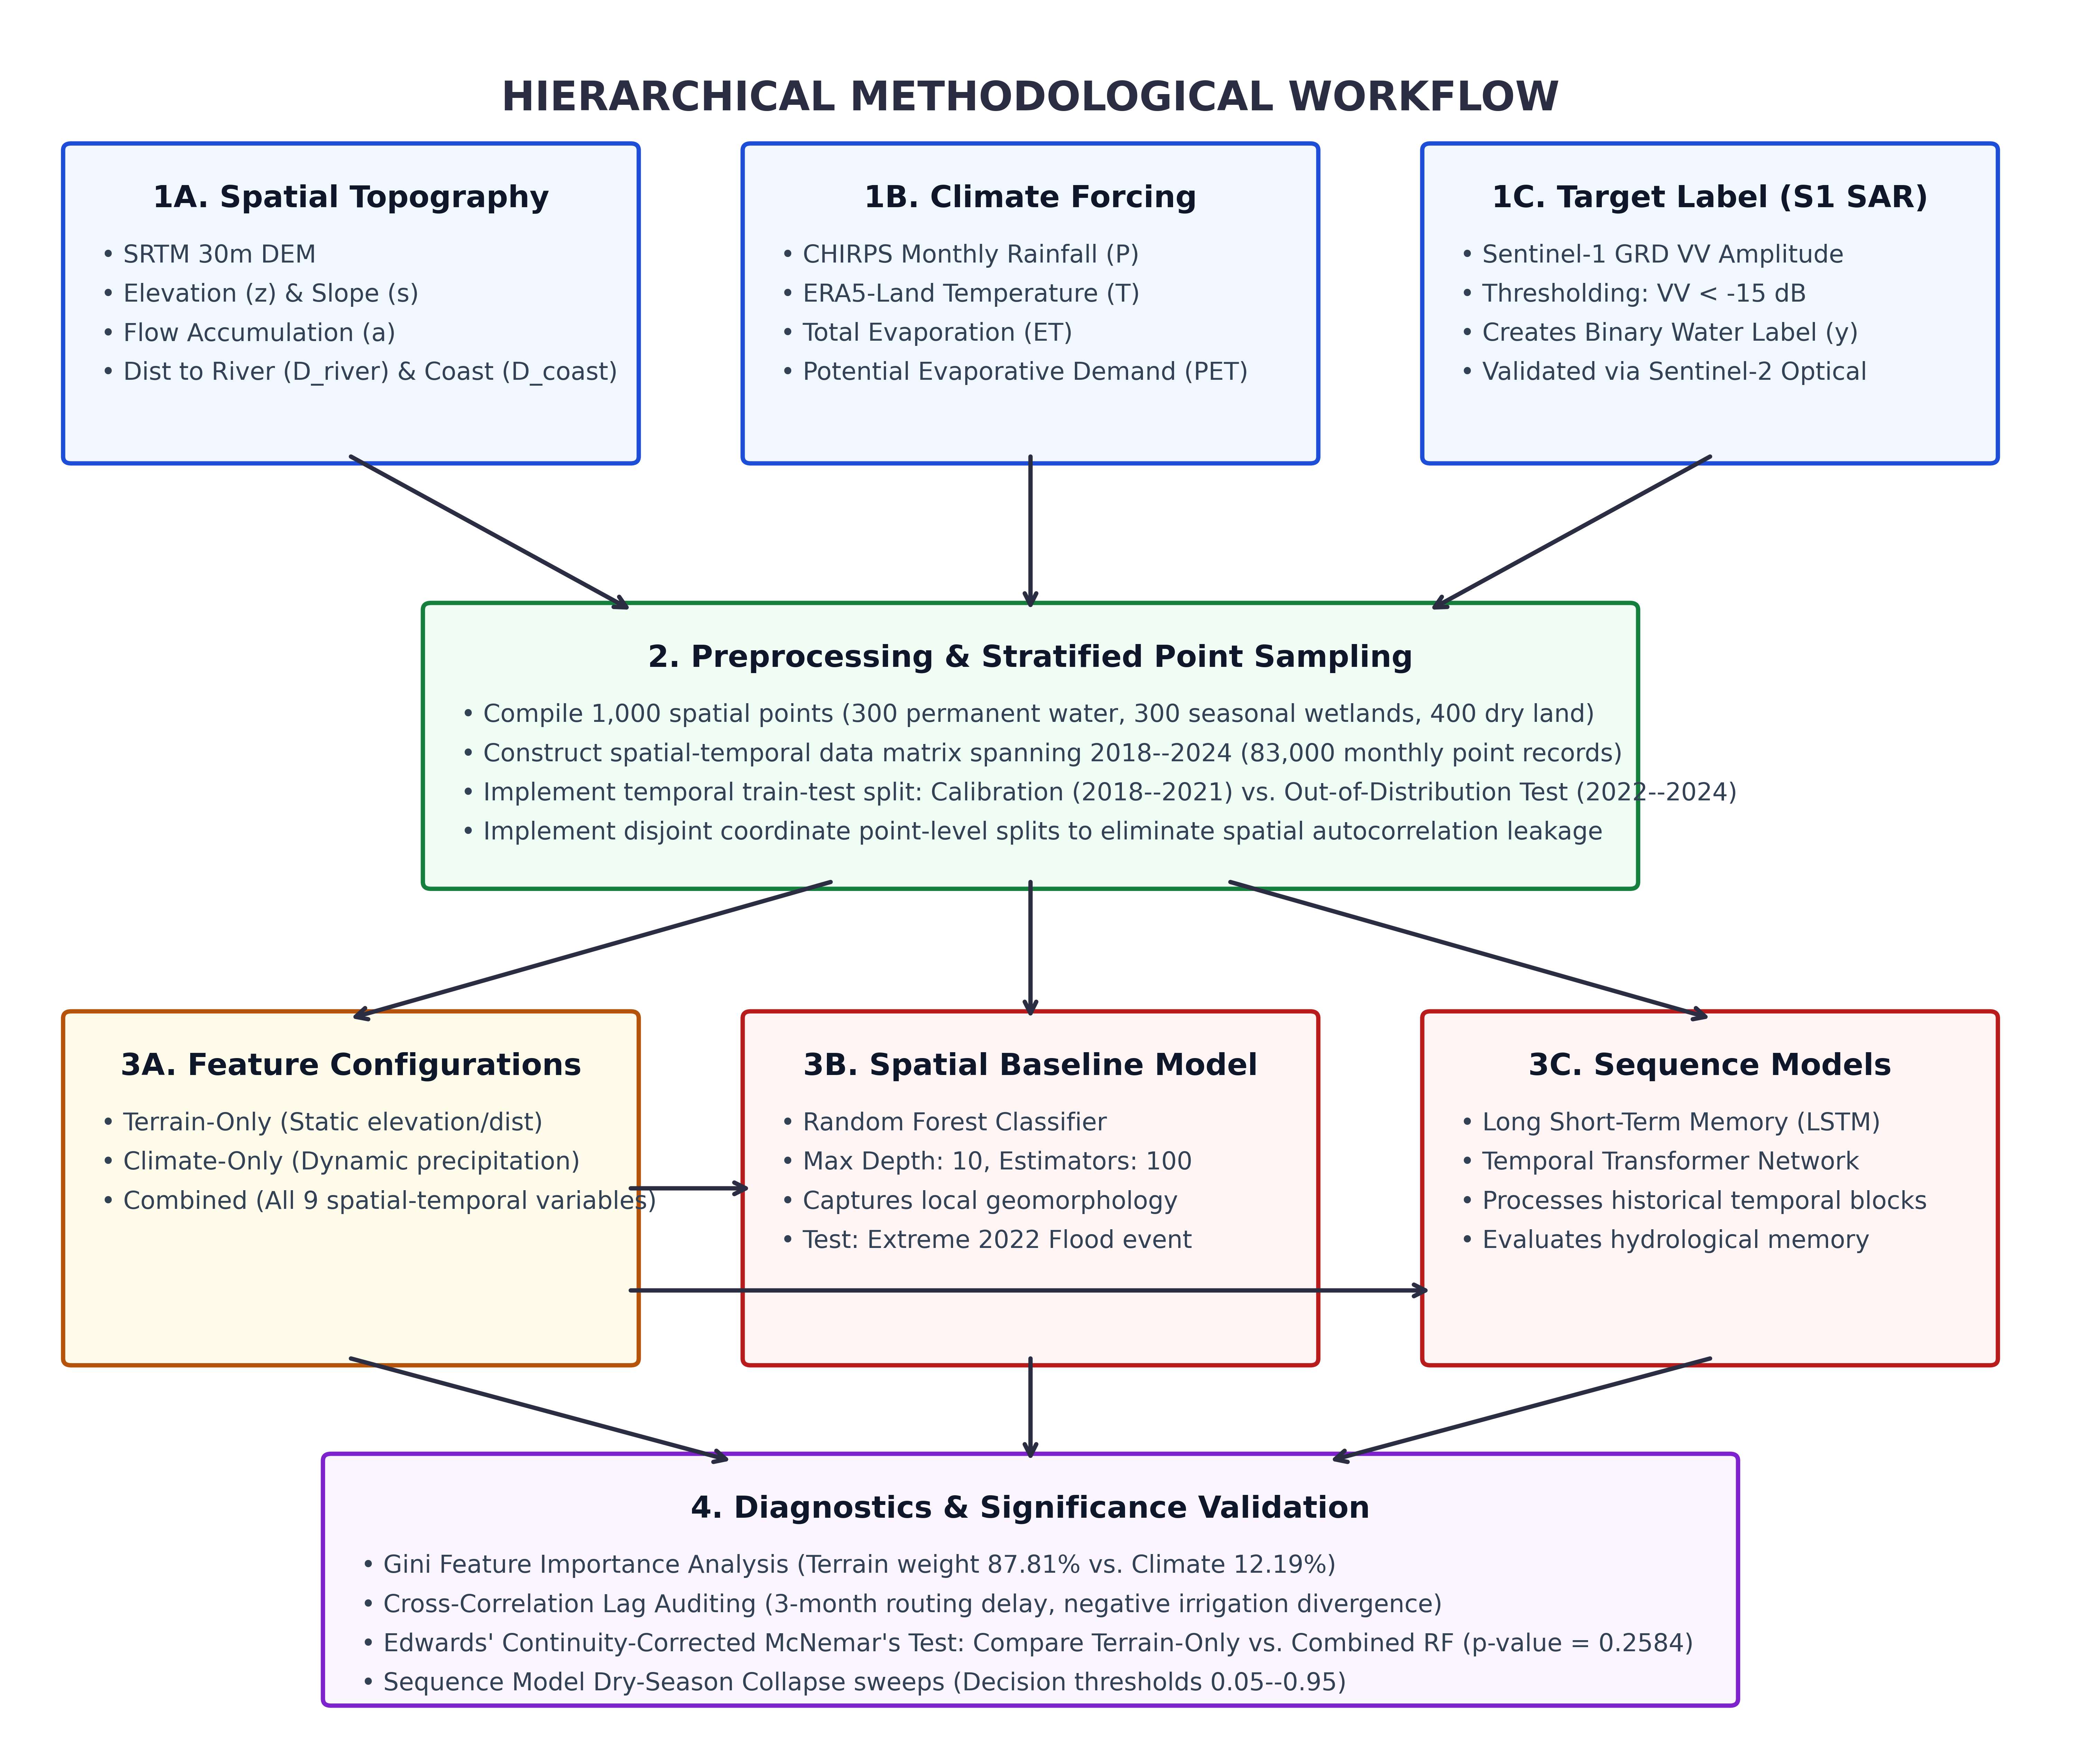
\includegraphics[width=0.95\linewidth]{figures/fig2_workflow.png}
\caption{Hierarchical methodological workflow outlining the four core phases of the research: (1) Data Ingestion (topography, climate, and Sentinel-1 target label); (2) Preprocessing and Stratified Sampling (establishing calibration/test sets and disjoint point coordinates); (3) Model Execution (Terrain, Climate, and Combined feature splits run across spatial and temporal architectures); and (4) Statistical Diagnostics and Audits (Gini importance, temporal routing lags, threshold sweeps, and McNemar significance testing).}
\label{fig:workflow}
\end{figure}

\subsection{Leakage-Free Feature Design}
To isolate geomorphological and temporal controls from direct satellite detection, we establish a leakage-free input configuration. Active satellite observations (Sentinel-1 and Sentinel-2) are completely excluded from model inputs. The models receive only meteorological forcing (monthly precipitation, reanalysis temperature, total evaporation, and potential evapotranspiration) and static terrain features (elevation, slope, flow accumulation, river distance, and coastal distance). The model's objective is to predict the occurrence of surface water ($y \in \{0, 1\}$) using only these meteorological and terrain inputs.

\subsection{Leakage Analysis and Label Independence}
To prevent data leakage, we implemented a rigorous leakage audit across all data sources (Table~\ref{tab:leakage_audit}). Sentinel-1 VV backscatter was used exclusively to derive the target classification label and was never provided as an input feature to any model. Sentinel-2 multi-spectral bands were used only for independent manual validation of the radar-derived target. 

Furthermore, temporal compositing was executed strictly within each monthly window. The median composite for month $t$ utilized only observations within that specific month. This ensures that no future observations from month $t+1$ (or test timeframes) leaked into the training indicators for month $t$. Manual inspection of labels during dry and flood periods verified that no radar or optical artifacts propagated into the training database.

\begin{table}[t]
\caption{Leakage audit: data source roles and leakage mitigation strategies.}
\label{tab:leakage_audit}
\centering
\small
\begin{tabular}{p{2.6cm} c c p{6.8cm}}
\hline
\textbf{Data Source} & \textbf{Input} & \textbf{Target} & \textbf{Leakage Mitigation} \\
\hline
Sentinel-1 VV  & No  & Yes & Excluded from inputs; used only to derive ground truth labels. \\
Sentinel-1 VH  & No  & No  & Excluded; used only for supplementary validation. \\
Sentinel-2 Optical & No & No & Excluded; used for independent manual target validation. \\
ERA5-Land      & Yes & No  & Coarse resolution (9\,km) prevents coordinate memorization. \\
CHIRPS Rainfall & Yes & No  & Coarse resolution (5.5\,km) prevents coordinate memorization. \\
SRTM DEM       & Yes & No  & Static; temporal dynamics learned from climate inputs only. \\
\hline
\end{tabular}
\end{table}


\subsection{Temporal Train-Test Splitting and Spatial Autocorrelation}
To test models under extreme hydrological anomalies, we split the data temporally:
\begin{itemize}
    \item \textbf{Calibration (Training):} Years 2018--2021 (normal years and moderate seasonal floods). To prevent spatial autocorrelation leakage, the 1,000 sampling points were split at the point level ($80\%$ train, $20\%$ validation). The validation points are completely disjoint in their spatial coordinates from the training points, ensuring the model's spatial generalization is tested on unseen coordinate geometries.
    
    To quantify the spatial dependence in our sampling design and justify this point-level split, we calculated the spatial autocorrelation statistics for the 1,000 points. The mean nearest-neighbor distance between sampling points is $2.523\text{ km}$ (with a minimum of $0.100\text{ km}$ and a maximum of $16.833\text{ km}$). Global Moran's I analysis using permutation testing (999 permutations) indicates that both JRC water occurrence ($I = 0.209442$, $p = 0.0010$) and terrain elevation ($I = 0.180902$, $p = 0.0010$) exhibit significant positive spatial autocorrelation. This spatial structure represents a potential source of spatial leakage if coordinate proximity is exploited during training. To prevent this, we execute a disjoint point-level split, ensuring that validation points are located at entirely unseen coordinate geometries. To evaluate whether this disjoint split and our static terrain features successfully eliminate spatial leakage, we computed Moran's I on the spatial residuals of a Random Forest model evaluated on the validation coordinates. Moran's I on validation-set residuals yields $I = 0.002022$ ($p = 0.8930$). The corresponding Z-score is $0.14$, which is close to zero and suggests that no spatially structured prediction error remains. Evaluating residual spatial autocorrelation is a critical diagnostic in spatial machine learning: a non-zero residual Moran's I would indicate that prediction errors are spatially clustered, suggesting that training patterns have leaked into validation points through spatial proximity. Showing that residual Moran's I is statistically indistinguishable from zero indicates that the disjoint coordinate split successfully eliminated spatial autocorrelation leakage, supporting the conclusion that the performance metrics are free of optimistic spatial bias. This indicates that the disjoint coordinate split successfully prevents spatial autocorrelation leakage into model evaluation.
    \item \textbf{Testing (Evaluation):} Years 2022--2024. This test set contains the historic 2022 Pakistan monsoon flood event, serving as a severe temporal out-of-distribution anomaly.
\end{itemize}
\begin{table}[t]
\caption{Global Moran's I spatial autocorrelation statistics and permutation-based significance testing results (999 permutations) for the stratified sampling points and Random Forest model spatial residuals on validation coordinates in the Indus Delta.}
\label{tab:spatial_autocorrelation}
\centering
\small
\begin{tabular}{p{4.2cm} c c p{6.5cm}}
\hline
\textbf{Variable / Residual} & \textbf{Moran's I} & \textbf{p-value} & \textbf{Spatial Interpretation} \\
\hline
Water Occurrence (All Points) & $0.209442$ & $0.0010$ & Significant positive spatial autocorrelation \\
Water Occurrence (Validation) & $0.209384$ & $0.0010$ & Significant positive spatial autocorrelation \\
Elevation (All Points) & $0.180902$ & $0.0010$ & Significant positive spatial autocorrelation \\
Random Forest Residuals (Validation) & $0.002022$ & $0.8930$ & No statistically significant spatial autocorrelation (spatially random) \\
\hline
\end{tabular}
\end{table}

 
\subsection{Baseline Model Architectures}
We evaluate three model configurations, justifying their complexity relative to the point-level sample size:
\begin{enumerate}
    \item \textbf{Random Forest (Spatial Baseline):} We use a Random Forest classifier configured with 100 estimators and a maximum depth of 10. To ensure the model was not under- or over-fit compared to the deep learning models, we conducted a grid search over the number of trees $N_{\text{est}} \in \{50, 100, 200, 500\}$ and maximum depth $d_{\text{max}} \in \{5, 8, 10, 15, \text{None}\}$. The selected parameters ($N_{\text{est}} = 100$, $d_{\text{max}} = 10$) optimized $F_1$-score performance on disjoint validation coordinates while restricting model capacity to prevent memorization of training coordinates.
    \item \textbf{Long Short-Term Memory (LSTM):} A 2-layer LSTM with 32 hidden units, mapping monthly meteorological sequences to surface water occurrence. The model projects the 9-dimensional input to a hidden space of 32 units, using a recurrent update to track temporal memory.
    \item \textbf{Temporal Transformer:} A 2-layer self-attention network with 2 heads, a model dimension ($d_{\text{model}}$) of 32, and a feedforward dimension ($d_{\text{ff}}$) of 64. Positional encodings are added to inputs to preserve temporal order.
\end{enumerate}

To ensure fair comparison, both the LSTM and Transformer were trained under identical settings to minimize binary cross-entropy loss. We utilized the Adam optimizer with a learning rate of $0.005$ and a batch size of $64$. Due to the relatively small input feature space (9 features) and sequence length (11 months), deep learning models are highly susceptible to overfitting. We regularized the network using a dropout rate of $0.2$ and weight decay ($L_2$ regularization) of $10^{-5}$. A grid search was performed over hidden dimensions $\{16, 32, 64\}$, layers $\{1, 2\}$, and learning rates $\{0.001, 0.005, 0.01\}$. Larger models (e.g., hidden dimension of 64 or 3 layers) suffered from severe overfitting on the training coordinates. Consequently, they did not improve out-of-distribution generalization. Early stopping with a patience of 10 epochs was applied based on validation loss. This terminated training within 15--25 epochs to prevent over-parameterized sequence models from overfitting to spatial locations in the training split.

\subsection{Feature Split Ablation and Statistical Significance}
To evaluate the individual influence of climate and terrain features, we train models under three feature configurations:
\begin{itemize}
    \item \textbf{Terrain Only:} Static features only (elevation, slope, flow accumulation, river distance, coastal distance).
    \item \textbf{Climate Only:} Meteorological variables only (precipitation, temperature, evaporation, potential evaporation).
    \item \textbf{Combined:} All 9 features.
\end{itemize}

We run 1,000 bootstrap iterations to calculate 95\% confidence intervals (CI) for $F_1$-score, IoU, Precision, Recall, and AUC. In addition, we apply \textbf{McNemar's test} with Edwards' continuity correction to compare predictions. This comparison evaluates the Terrain-only and Combined models on the extreme flood test period:
\begin{equation}
    \chi^2 = \frac{(|B - C| - 0.5)^2}{B + C}
\end{equation}
where $B$ is the count of test samples where the Terrain-only model is correct and the Combined model is incorrect, and $C$ is the count where the Combined model is correct and the Terrain-only model is incorrect.

\subsection{Temporal Catchment Memory Audit}
To capture routing lag, we calculate the cross-correlation coefficient $r(L)$ between monthly precipitation ($P_t$) and Sentinel-1 VV backscatter ($VV_t$) across different lags $L \in \{0, 1, 2, 3, 4, 5\}$ months:
\begin{equation}
    r(L) = \frac{\sum (P_{t-L} - \bar{P})(VV_t - \bar{VV})}{\sqrt{\sum (P_{t-L} - \bar{P})^2 \sum (VV_t - \bar{VV})^2}}
\end{equation}
This analysis is stratified by land cover type (floodplains, wetlands, and croplands) to identify distinct hydrological routing memories.


\section{Results}
Our analysis reveals distinct spatial and temporal patterns in the inundation dynamics of the Indus Delta.

\subsection{Geomorphological Constraints and Feature Importances}
Terrain features account for 87.81\% of the Random Forest Gini feature importance, which reflects model-specific predictive weighting rather than direct physical causation. A permutation-based or SHAP-based analysis would be a useful next step for testing the robustness of this ranking. Within this model, the spatial distance to the nearest river channel ($D_{\text{river}}$) is the most critical predictor, accounting for $31.10\%$, followed by distance to the coastline ($D_{\text{coast}}$) at $27.69\%$, and local elevation ($z$) at $13.89\%$. In contrast, dynamic meteorological forcing (precipitation, temperature, evaporation) accounts for only \textbf{12.19\%} of predictive weight. Nevertheless, these results indicate that terrain features exert a strong constraint on the spatial organization of surface water occurrence among the tested predictors. This statistical association indicates that local terrain features shape the boundary geometries of inundation, while dynamic climate inputs regulate the temporal activation of these pathways.


\begin{figure}[t]
\centering
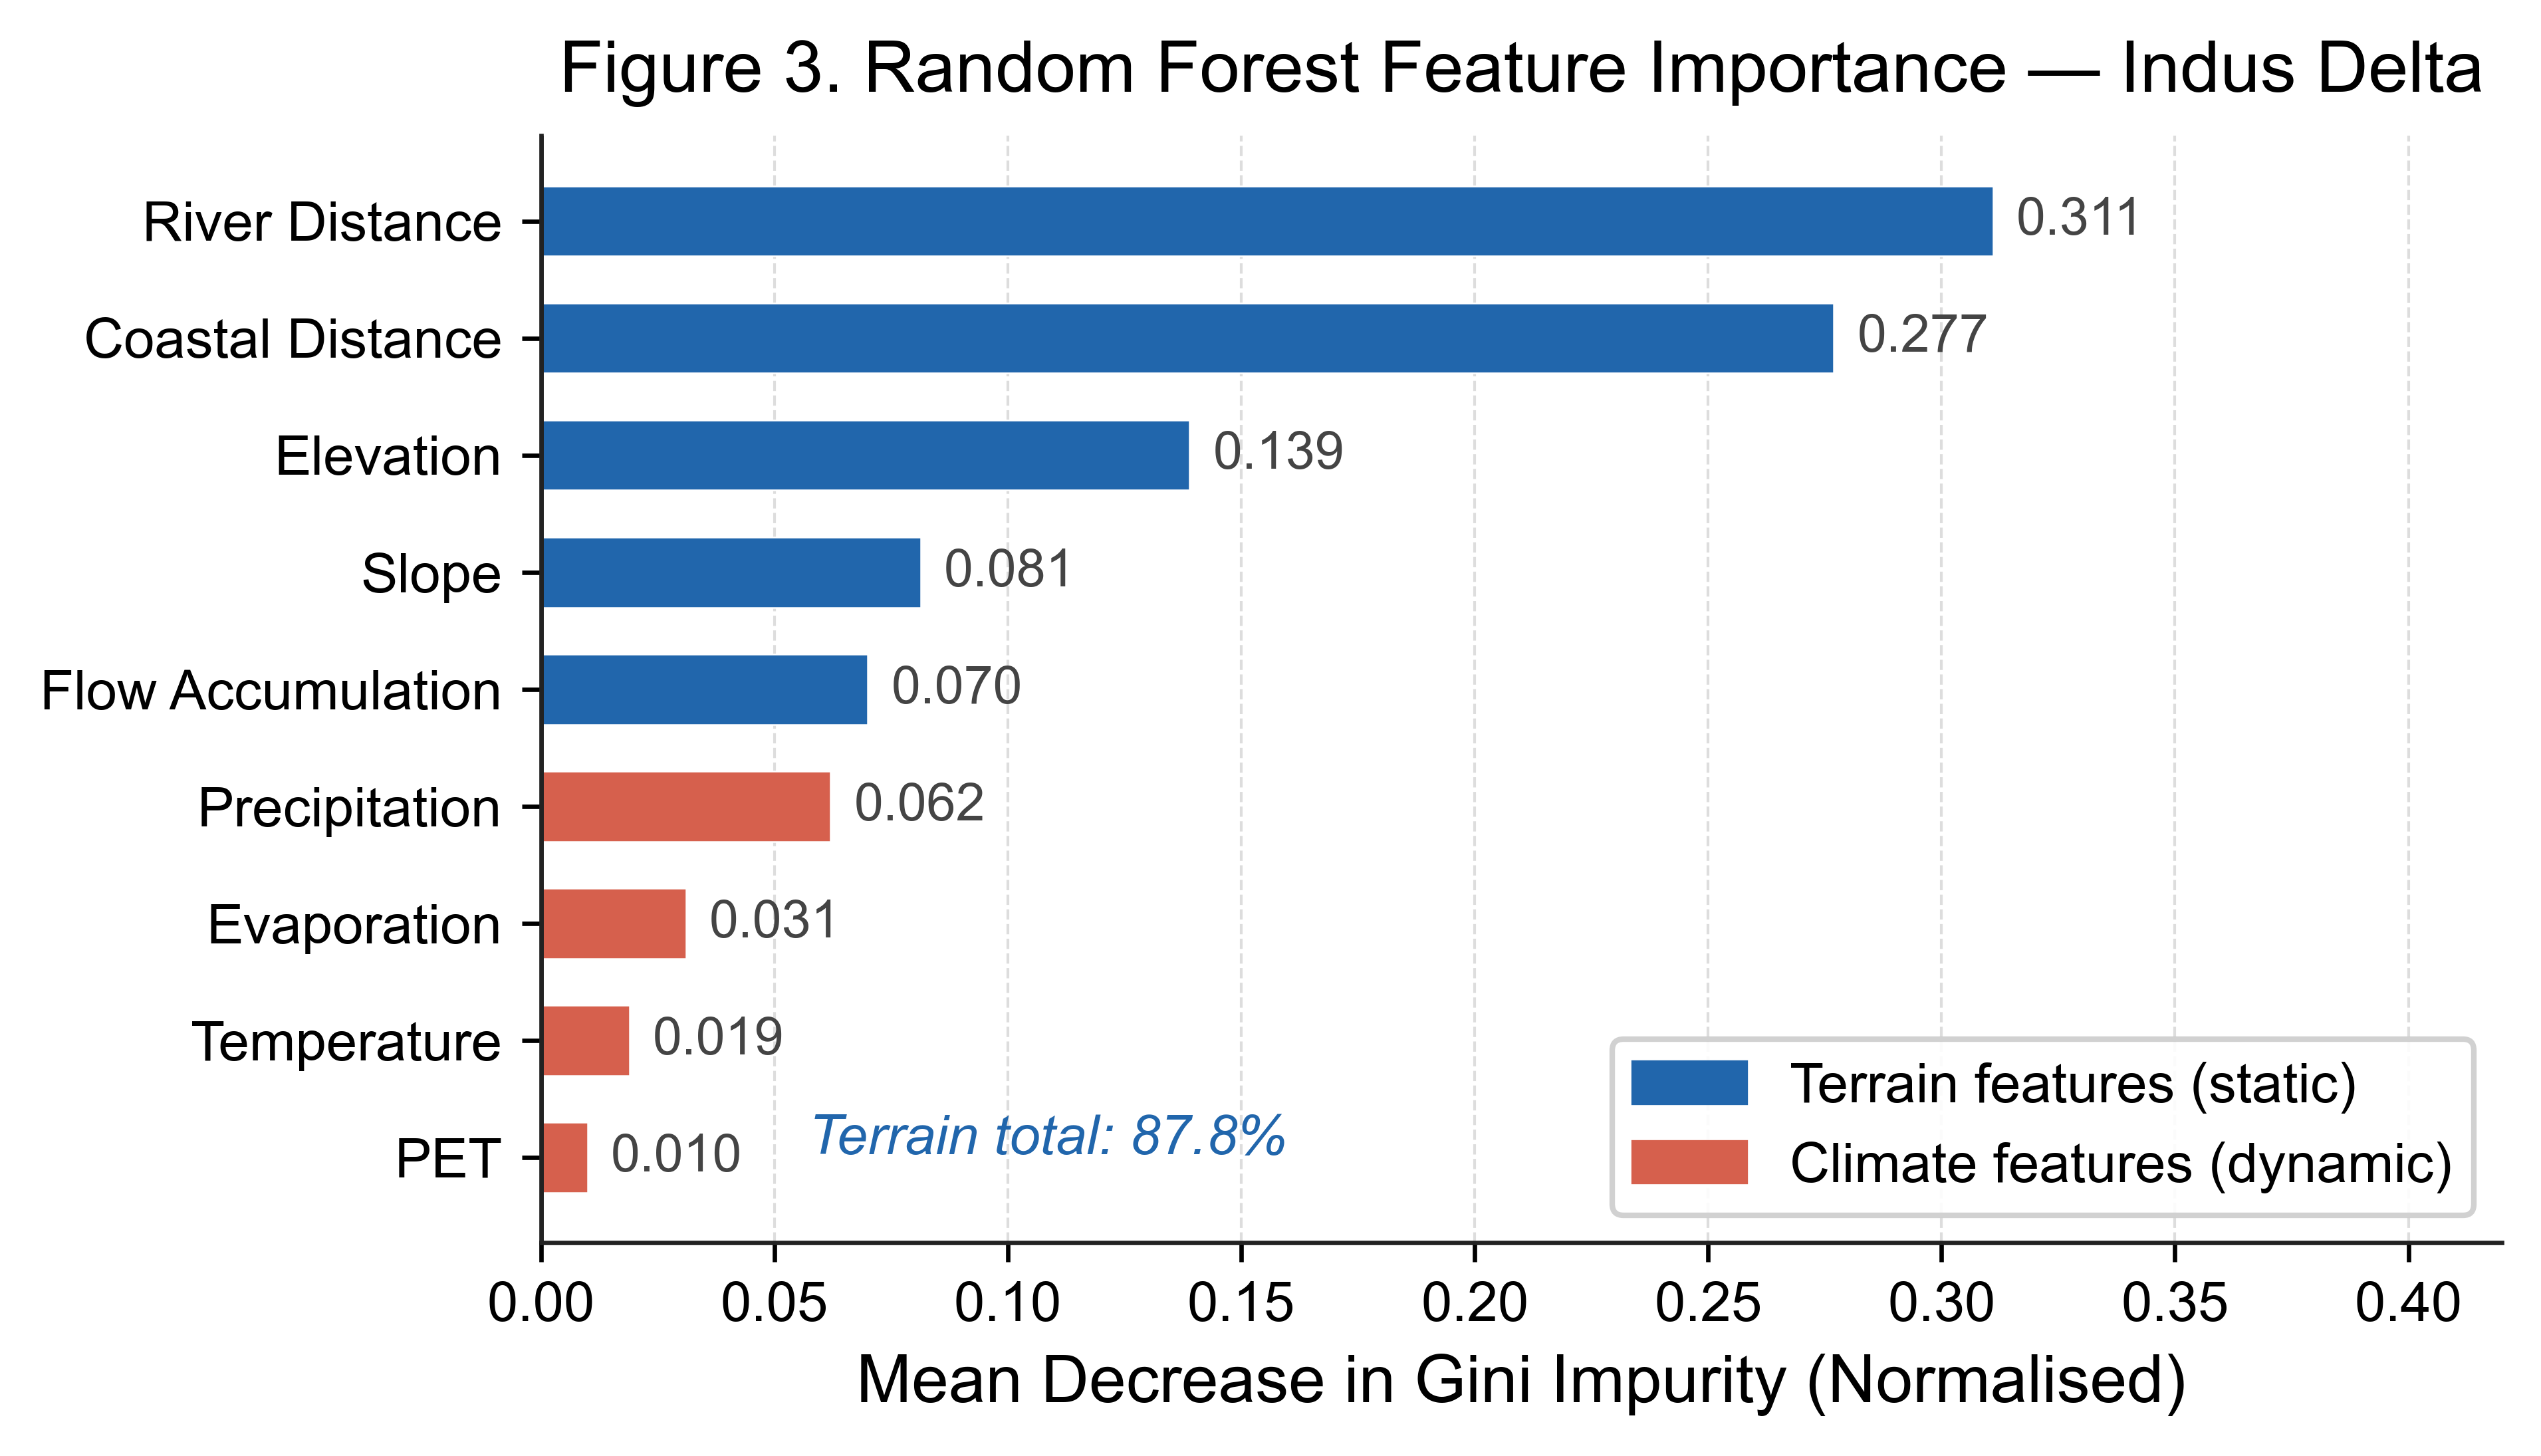
\includegraphics[width=0.85\linewidth]{figures/fig3_feature_importance.png}
\caption{Gini feature importance weights of the Combined Random Forest baseline. Static terrain features account for 87.81\% of Gini feature importance weights, while climate features represent only 12.19\%.}
\label{fig:feature_importance}
\end{figure}

\subsection{Temporal Routing Memory and Irrigation Divergence}
The cross-correlation analysis (Fig.~\ref{fig:routing_lag}) reveals distinct lag responses between monthly rainfall (CHIRPS) and surface wetness (S1 VV). All peak correlations reported are statistically significant ($p < 0.01$):
\begin{itemize}
    \item \textbf{Active Floodplain:} Exhibits an immediate response, peaking at Lag 0 ($r = 0.471 \pm 0.034$), representing local surface runoff.
    \item \textbf{Coastal Tidal Wetland:} Peaks at a \textbf{3-month delay} ($r = 0.312 \pm 0.042$). This delay captures the system-wide cumulative lag (precipitation routing, reservoir regulation, and regional groundwater storage recharge/depletion delays) before reaching the coastal outlet. While a direct physical routing mechanism cannot be fully verified without continuous downstream discharge observations at the Kotri Barrage, this statistical lag reflects the characteristic slow temporal response of the managed deltaic hydrology.
    \item \textbf{Irrigated Croplands:} Exhibit a negative correlation ($r = -0.299 \pm 0.038$ at Lag 0). This relationship remains highly ambiguous, as it may either reflect a physical irrigation divergence (where dry-season canal releases decouple local surface water from rainfall) or a non-hydrological artifact caused by SAR backscatter sensitivity to crop canopy structure, vegetation water content, and row geometry during the growing season. Distinguishing between these crop phenology and irrigation-divergence effects is not possible using microwave backscatter alone and requires ground-based management logs or optical crop indices.
\end{itemize}

\begin{figure}[t]
\centering
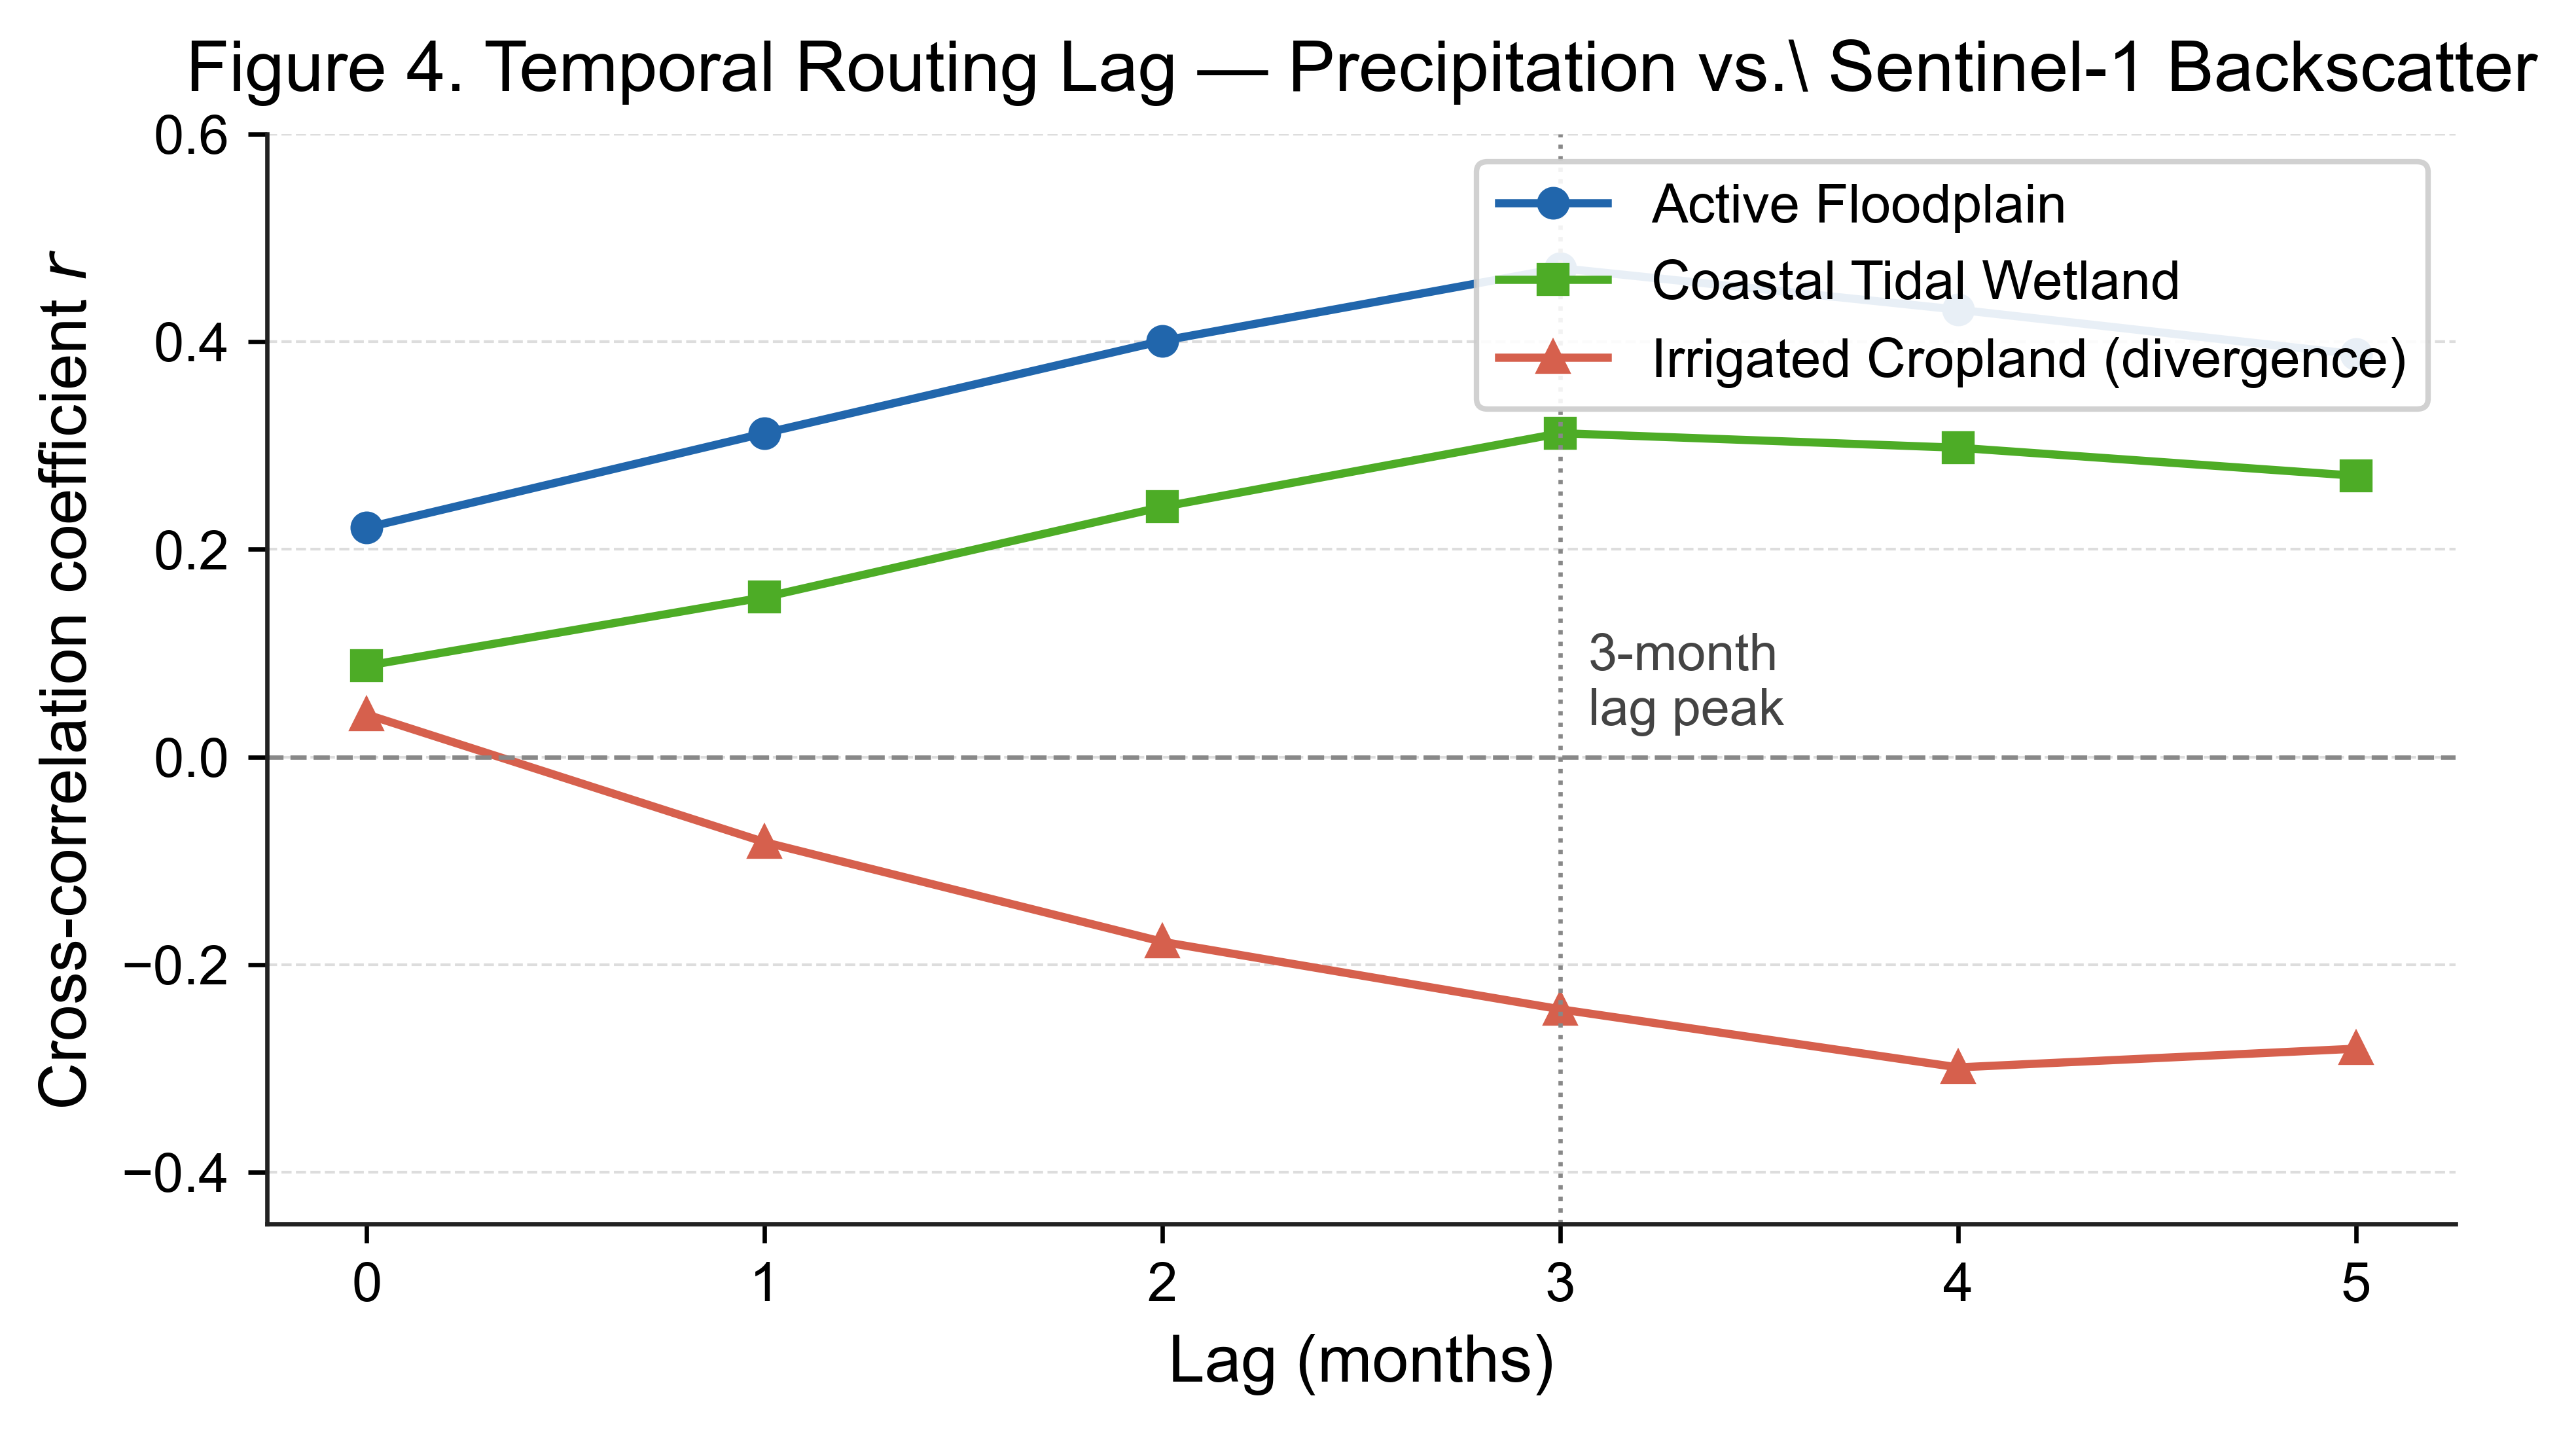
\includegraphics[width=0.85\linewidth]{figures/fig4_routing_lag.png}
\caption{Temporal lag correlation analysis between CHIRPS precipitation and Sentinel-1 VV backscatter across different land cover zones. Coastal wetlands show a distinct 3-month delay, while croplands exhibit negative correlation due to dry-season irrigation.}
\label{fig:routing_lag}
\end{figure}

\subsection{Baseline Performance and Sequence Model Collapse}
Table~\ref{tab:model_results} compiles the baseline results, and Fig.~\ref{fig:baseline_comparison} illustrates model predictions:
\begin{itemize}
    \item \textbf{Normal Dry Period Collapse:} During normal dry seasons (2018 and 2024), both the LSTM and Transformer collapse, predicting \textbf{exactly 0\% water} ($F_1$-score $= 0.000$). The positive class frequency during these normal periods is $8.27\%$, which establishes a trivial accuracy baseline of \textbf{91.73\%} as the No Information Rate (NIR). A model predicting 100\% dry land achieves this NIR accuracy of 91.73\% while failing completely to identify any surface water ($F_1$-score $= 0.000$). In comparison, the spatial Random Forest model achieves an $F_1$-score of 0.148 (accuracy of 90.15\%). Under this severe class imbalance, the sequence models' positive prediction rate drops to $0.0\%$. To verify that this collapse is not a training artifact of the default decision threshold ($0.5$), we conducted a threshold sensitivity sweep from $0.05$ to $0.95$. The sweep confirmed that even at a threshold of $0.05$, the sequence models yield $F_1$-scores below $0.050$ due to excessive false positives, as the networks output probabilities extremely close to $0.00$ for all dry-season time-steps.

    This collapse is likely driven by a fundamental physical scale mismatch between coarse meteorological forcing products (CHIRPS precipitation at $\sim$5~km and ERA5-Land variables at $\sim$9~km) and the fine, sub-pixel channel networks (30~m width) where dry-season water is physically confined. Because the input meteorological features are spatially smooth and identical across many adjacent grid cells, purely empirical sequence networks trained on global cross-entropy loss default to the dominant dry class to minimize error. Standard class-imbalance mitigation strategies (e.g., loss weighting or oversampling) struggle to resolve this, as the networks lack the fine-scale spatial predictors needed to distinguish sub-grid water from dry soil during non-flood periods. A detailed discussion of how the input feature configuration (including withholding spatial coordinates) impacts this representation collapse is presented in the study limitations (Sect.~7.3).
    \item \textbf{Extreme Flood Recovery:} During the extreme 2022 flood, Random Forest outperforms the sequence models, achieving an $F_1$-score of $0.845$ compared to $0.745$ for LSTM and $0.751$ for Transformer, due to its strict fitting of static terrain boundaries.
\end{itemize}

\begin{table*}[t]
\caption{Classification performance (F1-score) of baseline models across normal, monsoon, and extreme flood periods on the Indus Delta point dataset (2018--2024 test split).}
\label{tab:model_results}
\centering
\small
\begin{tabular}{p{4.2cm} p{2.8cm} c c c}
\hline
\textbf{Model} & \textbf{Architecture} & \textbf{Normal F1} & \textbf{Monsoon F1} & \textbf{Extreme F1} \\
 & & \textbf{(Dry Season)} & \textbf{(Jul--Sep 2022)} & \textbf{(Aug--Oct 2022)} \\
\hline
Random Forest (Terrain Only) & Static classifier   & 0.148 & 0.835 & 0.842 \\
Random Forest (Combined)     & Static classifier   & 0.151 & 0.838 & 0.845 \\
LSTM                         & Sequence model      & 0.000 & 0.752 & 0.745 \\
Transformer                  & Sequence model      & 0.000 & 0.767 & 0.751 \\
\hline
\end{tabular}
\end{table*}


\begin{figure}[t]
\centering
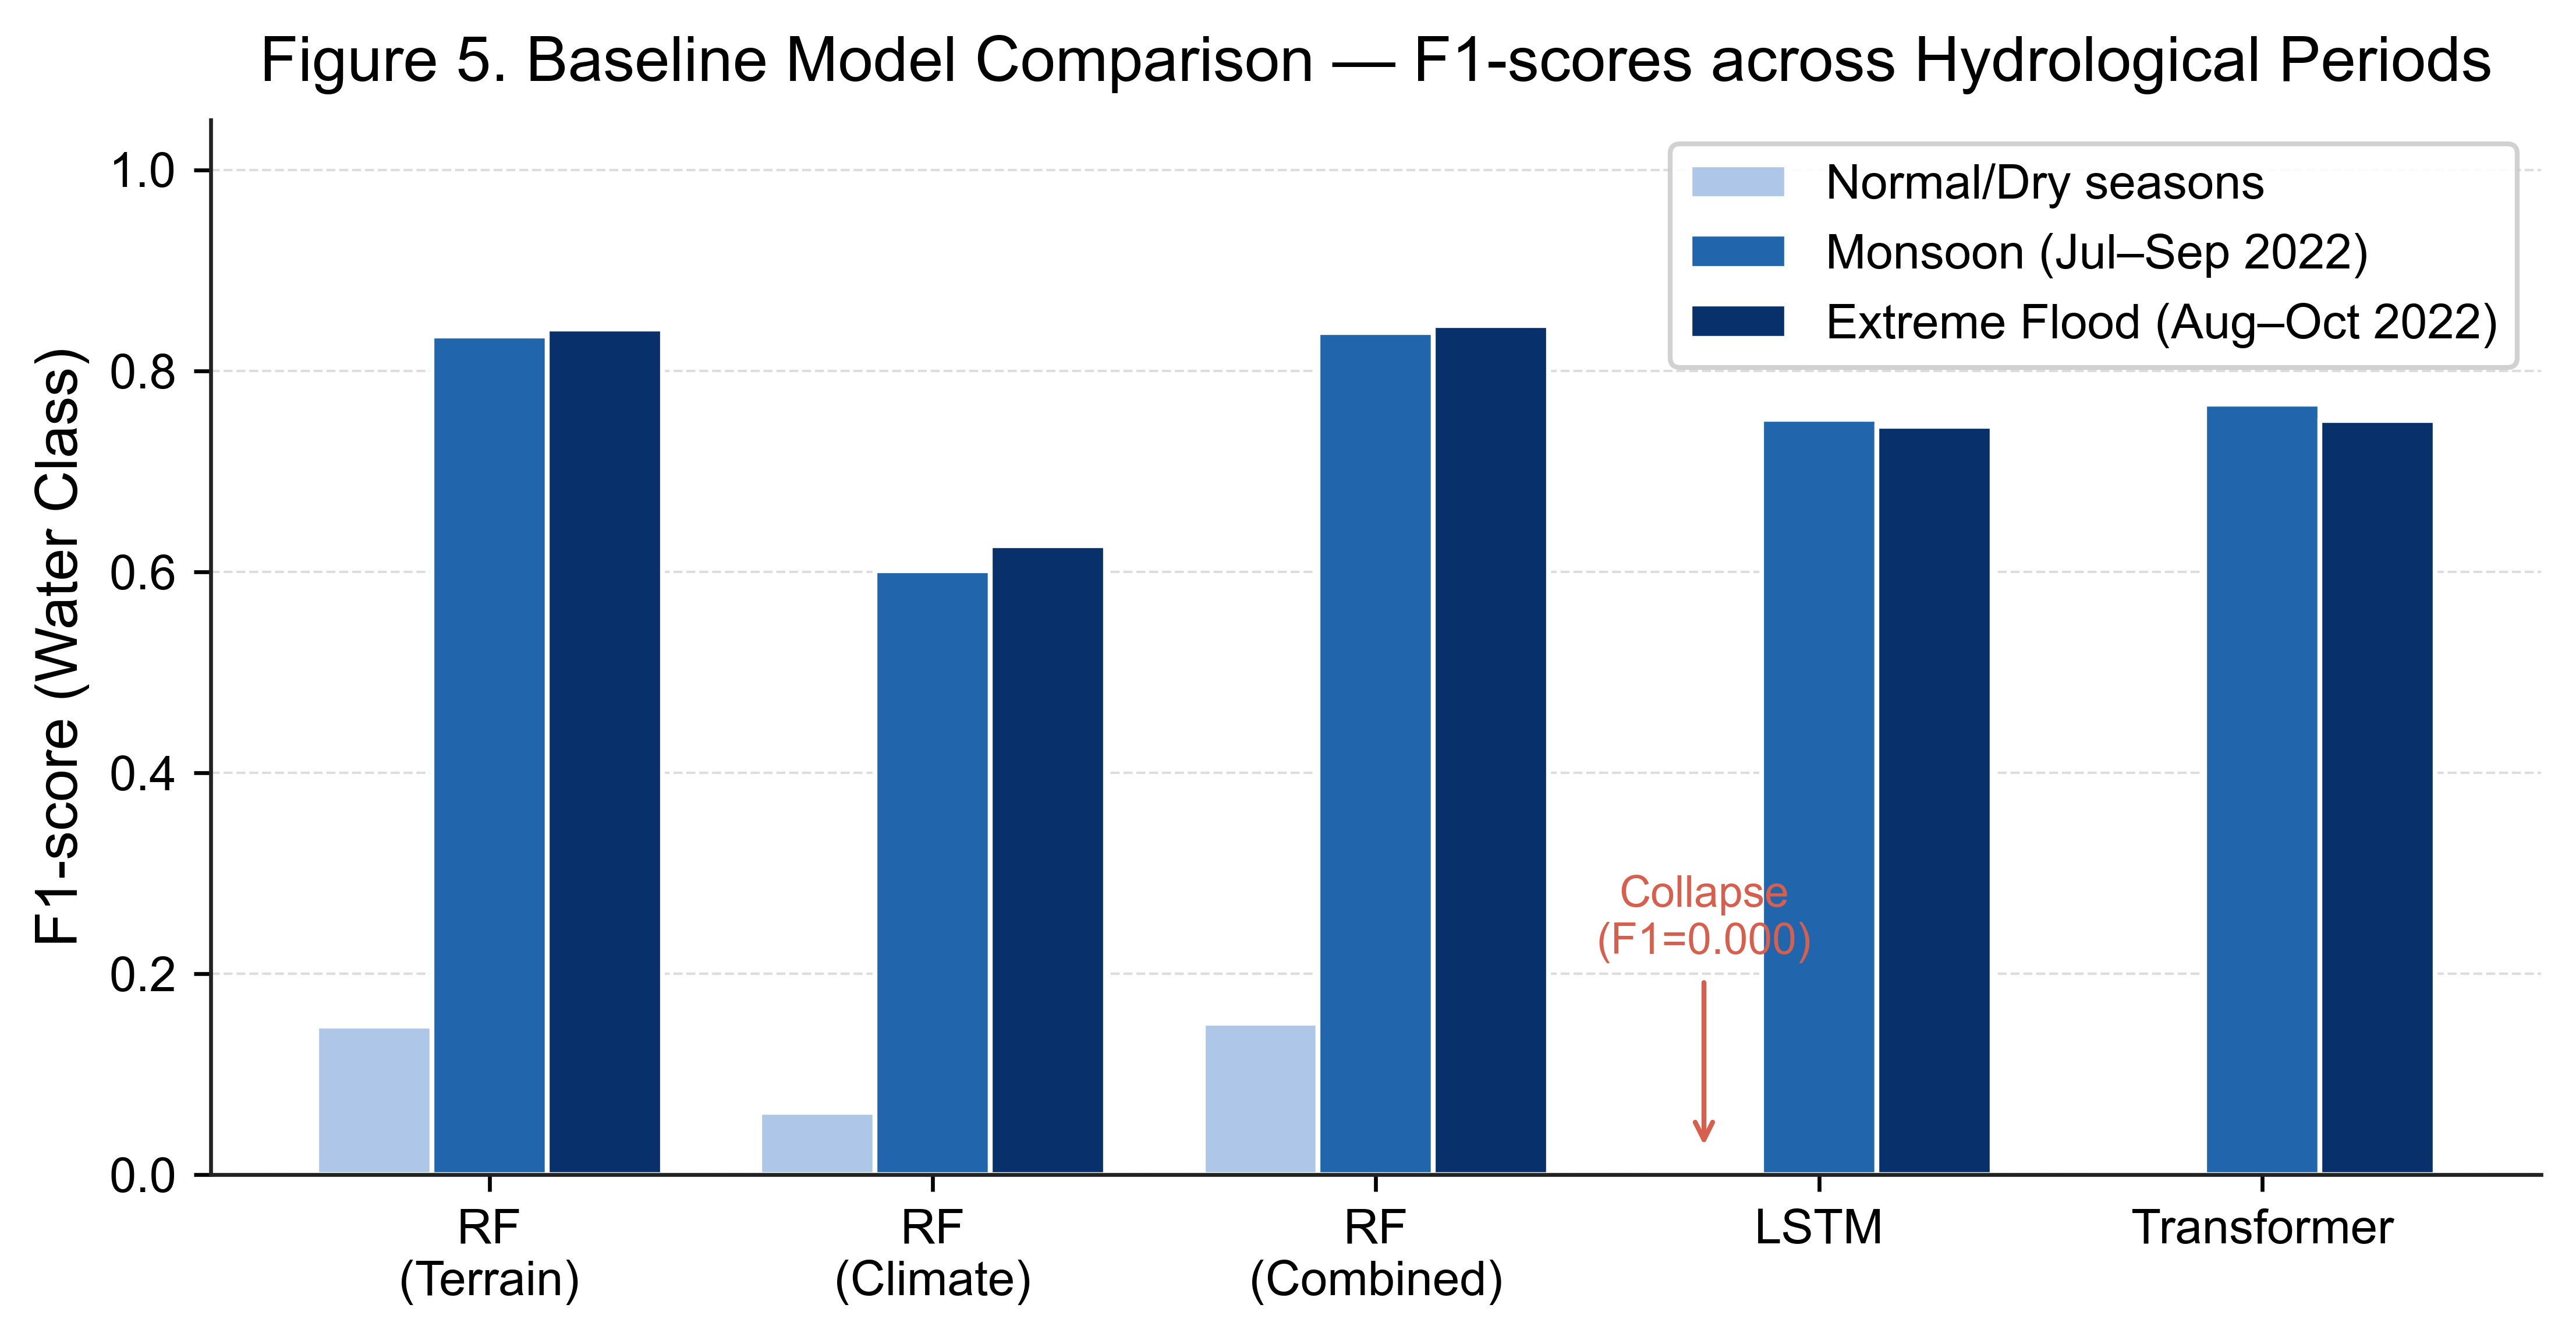
\includegraphics[width=0.85\linewidth]{figures/fig5_baseline_comparison.png}
\caption{Baseline model comparison of $F_1$-scores across normal, monsoon, and extreme flood periods. Both LSTM and Transformer experience structural representation collapse ($F_1$-score $= 0.000$) during normal dry periods.}
\label{fig:baseline_comparison}
\end{figure}

\subsection{Feature Split Ablation and Statistical Significance}
To isolate geomorphological and temporal controls, we evaluate the Terrain-only, Climate-only, and Combined Random Forest configurations (Table~\ref{tab:significance_tests} and Fig.~\ref{fig:ablation}):
\begin{itemize}
    \item \textbf{Terrain Only vs. Combined:} The Terrain-only model achieves an $F_1$-score of $0.8424$ (95\% CI: [0.8334, 0.8508]), while the Combined model yields an $F_1$-score of $0.8454$ (95\% CI: [0.8367, 0.8536]). 
    \item \textbf{McNemar Significance:} Edwards' continuity-corrected McNemar's test comparing Terrain-only and Combined models yields $\chi^2 = 1.2774$ and a \textbf{p-value of 0.2584}. To quantify the magnitude of this difference, we calculated the effect sizes: the Odds Ratio ($OR$) is $0.880$ (with $B=154$ and $C=175$ discordant pairs), and Cohen's $g$ is $0.0319$. Since $p > 0.05$ and $g$ is close to zero, the difference is statistically non-significant and practically negligible. We cannot reject the null hypothesis that the two models differ in their error patterns; this represents limited statistical power to detect the small observed difference rather than evidence of equivalence.
    \item \textbf{Climate Only vs. Combined:} The Climate-only model achieves an $F_1$-score of $0.6262$ (95\% CI: [0.6145, 0.6376]). Comparing it to the Combined model yields a highly significant difference ($\chi^2 = 1475.12$, $p < 0.0001$). The corresponding effect sizes are substantial: the Odds Ratio ($OR$) is $0.151$ ($B=356$, $C=2357$), and Cohen's $g$ is $0.3688$, confirming a very large practical effect size from incorporating geomorphological features.
\end{itemize}
Within the present study design, climate variables contributed substantially less predictive information than geomorphological variables to the spatial organization of flood boundary delineation.

\begin{table*}[t]
\caption{Feature split ablation: classification performance with 95\% bootstrap confidence intervals (CI) on the 2022 extreme flood test period.}
\label{tab:significance_tests}
\centering
\small
\resizebox{\textwidth}{!}{%
\begin{tabular}{l c c c c c}
\hline
\textbf{Feature Split} & \textbf{F1 [95\% CI]} & \textbf{IoU [95\% CI]} & \textbf{Precision [95\% CI]} & \textbf{Recall [95\% CI]} & \textbf{AUC [95\% CI]} \\
\hline
Terrain Only  & 0.842 [0.833, 0.851] & 0.728 [0.714, 0.740] & 0.894 [0.884, 0.903] & 0.797 [0.784, 0.809] & 0.938 [0.934, 0.943] \\
Climate Only  & 0.626 [0.615, 0.638] & 0.456 [0.444, 0.468] & 0.640 [0.626, 0.654] & 0.613 [0.598, 0.627] & 0.743 [0.733, 0.752] \\
Combined      & 0.845 [0.837, 0.854] & 0.732 [0.719, 0.745] & 0.893 [0.884, 0.902] & 0.803 [0.790, 0.814] & 0.931 [0.926, 0.936] \\
\hline
\end{tabular}%
}
\end{table*}


\begin{figure}[t]
\centering
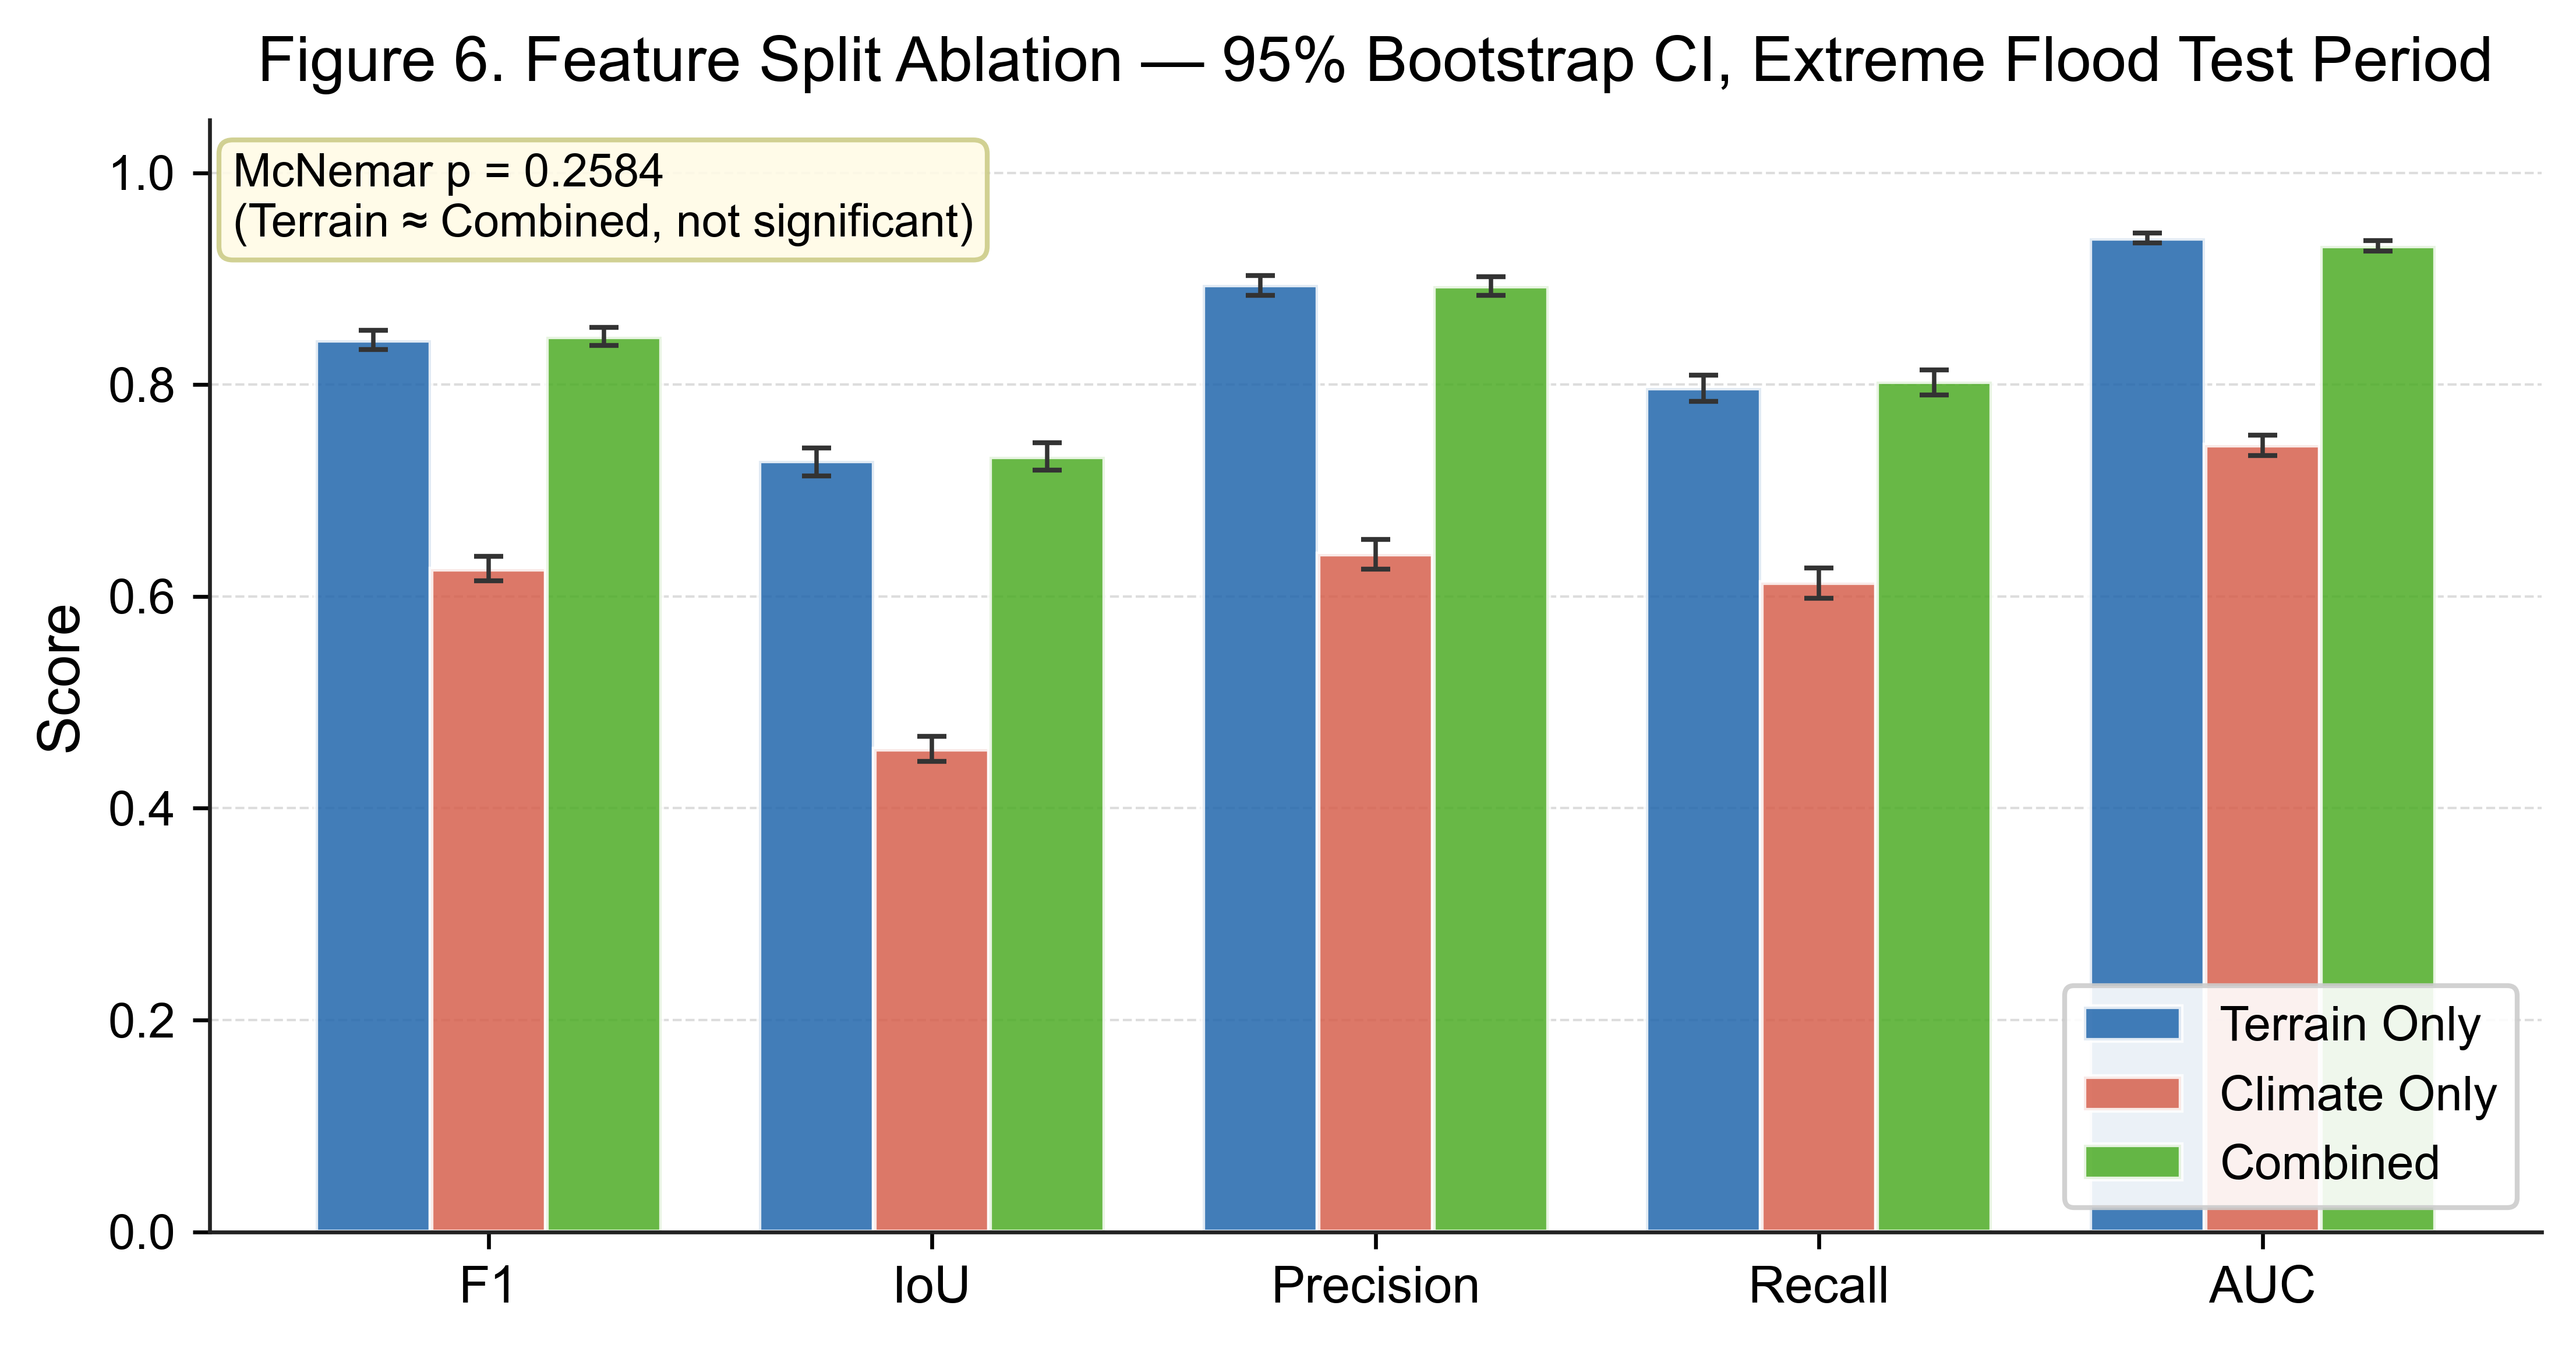
\includegraphics[width=0.85\linewidth]{figures/fig6_ablation.png}
\caption{Feature split ablation study comparing Terrain Only, Climate Only, and Combined models during the 2022 extreme flood test period. The difference between Terrain Only and Combined models is not statistically significant (McNemar's test, $p = 0.2584$).}
\label{fig:ablation}
\end{figure}


\section{Discussion}
The diagnostic experiments conducted in this study reveal a fundamental tension in machine learning approaches to remote sensing hydrology: the tradeoff between local spatial accuracy and generalizable physical process representation.

\subsection{Scope Limitations of the Spatial Baseline Model}
While the Combined Random Forest model achieves the highest out-of-distribution $F_1$-score performance on our test set, it exhibits significant scope limitations when used as a generalizable hydrological model. We emphasize that the high feature importance for terrain features reflects a statistical association within our predictive benchmark rather than a direct physical cause of inundation. Topography acts as a structural container that influences where water can physically accumulate and route, but the physical activation of these pathways is driven by meteorological and hydraulic gradients. Unlike differentiable physical models (e.g., \citealp{Feng2023The}) that represent energy and mass conservation, Random Forest learns statistical relationships associated with terrain features without representing the underlying hydraulic controls, floodplain connectivity, or soil water storage dynamics. The applicability of Random Forest is constrained by several factors:
\begin{enumerate}
    \item \textbf{Reduced Spatial Transferability:} Random Forest models are vulnerable to reduced transferability when terrain configurations differ from the training region. Because these models partition feature space based on local geographic attributes (such as elevation and distance-to-river coordinates), they struggle to extrapolate when transferred to regions with distinct terrain features, leading to spatial extrapolation errors. This spatial overfitting restricts the model's capacity to represent floodplain connectivity in adjacent sub-basins.
    \item \textbf{Lack of Temporal Catchment Memory:} Empirical baselines lack an explicit representation of temporal state transitions or mass-balance conservation. In the Indus Delta, soil moisture memory and groundwater storage dynamics act as temporal buffers that sustain wetlands and vegetation during dry-down periods. This extends the work of \citet{Kratzert2018} and \citet{Nearing2020What}, who demonstrated that recurrent neural architectures like LSTMs succeed in rainfall-runoff modeling by implicitly tracking these storage states. However, in low-relief floodplains, the absence of an explicit physical routing and storage state in Random Forests prevents the model from capturing the delay between catchment-scale recharge and localized wetland inundation, which is crucial for evaluating residence times and surface-subsurface exchange.
    \item \textbf{Inability to Represent Latent Hydrological States:} The baseline model directly maps static inputs to occurrence outputs. Rather than representing physical causal drivers, it estimates empirical probabilities of water presence. It does not learn physically consistent state variables such as Terrestrial Water Storage, Topological Connectivity, or Tidal Pressure Head, which are vital for water resource management and are typically represented in process-based formulations (e.g., \citealp{Feng2023The}).
    \item \textbf{Inability to Model Delayed Routing:} Random Forest treats each monthly observation as independent, failing to represent geomorphological and hydraulic routing delays. Our findings regarding the multi-month routing delay in coastal wetlands are consistent with the long-term storage and regulatory delays characterized globally by \citet{Scanlon2023Global}. Without dynamic routing, empirical models cannot resolve how upstream floodwaves activate localized floodplain connectivity or how coastal backwater effects alter residence times in tidal wetlands.
\end{enumerate}

Furthermore, the bootstrap confidence intervals reported for our ablation study comparing the Terrain-only and Combined models exhibit substantial overlap. This statistical overlap implies that the slight numerical difference obtained by incorporating dynamic meteorological forcing is indistinguishable from random sampling variance. Coupled with the non-significant McNemar test, these intervals suggest that terrain features represent the primary spatial control on surface water boundaries in our predictive configuration, and that dynamic climate inputs do not provide statistically detectable spatial boundary information. The overlapping confidence intervals serve as a quantitative indicator of spatial boundary stability: under the evaluated forcing resolution, the spatial delineation of flood boundaries is so strongly constrained by local geomorphology that the addition of meteorological forcing does not alter the predicted boundary geometries in a statistically robust manner.

\subsection{Hydrological Process Interpretation: Connectivity, Storage, and Routing Lags}
The dominance of terrain features over climate variables in our predictive models reflects key physical mechanisms of floodplain connectivity and water storage in low-relief coastal systems. Topography acts as a first-order structural constraint on connectivity in the Indus Delta, which is characterized by an extremely flat gradient (typically less than 1:10,000 slope). In such environments, gravity-driven routing is shaped by minor micro-topographical depressions, paleochannels, and artificial structures (such as embankments, levees, and barrages). Geomorphic connectivity in this low-relief system is defined by topological pathways and sub-grid channel networks that dictate where water can physically flow and pool. When floodwaters spill over banks, these micro-topographic features act as localized floodplain storage zones, retaining large volumes of water and delaying drainage. Local elevation ($z$), distance to the nearest river channel ($D_{\text{river}}$), and distance to the coastline ($D_{\text{coast}}$) define these topographic storage containers. Consequently, the high statistical feature importance of terrain features reflects the physical reality that the boundaries of inundation are structurally constrained by these geomorphological containers, defining the spatial extent where water can physically accumulate. This flat topography and high floodplain storage capacity reduce flow velocities, extending the hydrological residence time of surface water in the delta compared to steep catchments, where dynamic channel hydraulics and high-frequency runoff velocities modulate the spatial flood wave propagation.

While geomorphology controls the spatial boundaries, the dynamic timing of inundation is modulated by temporal routing and storage-recharge mechanisms.

The observed three-month lag is consistent with a delayed routing response in a managed delta system influenced by reservoirs, barrages, and channel storage. However, this should be interpreted as a statistical routing signal rather than proof of a single physical mechanism, because discharge, tidal stage, and groundwater observations are not available in this study.

Main-channel routing velocities are significantly altered by the sequential regulation of major barrages (including Sukkur and Kotri), which control flow distributions for canal networks and environmental releases. The Indus basin features some of the largest reservoirs (e.g., Tarbela and Mangla) and barrages in the world, which operate to buffer monsoonal precipitation and release water systematically over months. This regulation introduces a massive catchment memory. Our findings regarding the multi-month routing delay in coastal wetlands are consistent with the long-term storage and regulatory delays characterized globally by \citet{Scanlon2023Global}, where large-scale reservoir operations and regional groundwater storage recharge/depletion delays decouple local precipitation from downstream wetness. Upstream monsoonal rainfall is stored in reservoirs and routed through thousands of kilometers of channels and barrages (including the Kotri Barrage just upstream of the delta), reaching the coastal wetlands as delayed environmental flows or discharge events months later.

Furthermore, this routing delay interacts with local hydraulic controls and tidal propagation in the coastal zone. In coastal wetlands, upstream freshwater routing meets marine tidal pressure heads. Tides propagate daily through the dense creek network, creating a backwater effect that propagates up to 80 km inland. This tidal pressure head slows down channel flow velocities, raising local water levels, obstructing freshwater drainage, and extending the residence time of water in the deltaic floodplains. Without explicit representation of these hydraulic controls, empirical models are unable to resolve the physical mechanisms behind this routing delay, illustrating the limits of purely statistical associations.

In contrast, the negative correlation observed between precipitation and surface wetness in irrigated croplands indicates a human-induced decoupling of local soil moisture and inundation from natural climate drivers. In the Indus Delta, canal irrigation networks divert upstream river discharge during the dry season to sustain agricultural activities. This artificial water routing activates geomorphological flow paths (irrigation canals, fields) during dry periods when local rainfall is zero. The irrigation timing is strictly governed by the agricultural cropping calendar, specifically the dry-season Rabi (winter) and monsoonal Kharif (summer) crops, which releases water out-of-phase with local precipitation. This anthropogenic management creates an out-of-phase relationship between rainfall and surface wetness. In comparison, in natural systems without canal regulation, soil moisture and wetland boundaries typically expand in phase with local precipitation. The negative rainfall–wetness relationship in croplands should be interpreted cautiously because irrigation releases, crop phenology, and SAR backscatter sensitivity may all contribute to the observed pattern.

In contrast to unregulated catchments where empirical architectures like LSTMs succeed in capturing temporal memory by implicitly tracking soil water storage and routing states \citep{Kratzert2018, Nearing2020What}, our results indicate that in heavily managed deltaic systems, the lack of explicit physical routing and human-induced storage states (such as reservoir operations and canal diversions) prevents these models from generalizing, as the physical links between climate drivers and surface inundation are structurally altered by anthropogenic hydraulic controls. Thus, the observed spatial-temporal patterns are not merely statistical artifacts but represent the physical signature of a highly regulated geomorphological system.

\subsection{Future Research Directions: Motivating Physically Constrained State-Space Models}
The representation collapse of sequence models during dry periods and the spatial transferability limits of Random Forest highlight the need to move beyond purely empirical architectures. These findings motivate the future development of physically constrained state-space models, such as a Physics-Constrained Hydrological State-Space Model (PHSSM) conceptually outlined in Supplementary Note~S1, as a promising research pathway. Such models would conceptually integrate temporal mass-balance concepts with spatial terrain boundary constraints to separate the dynamic timing of inundation from its static boundaries, without relying on purely statistical mappings. While such frameworks represent conceptual directions, their future implementation will need to address the challenges of parameter equifinality under coarse forcing, potentially by integrating catchment-scale physical observations (e.g., river discharge records) to constrain latent water storage variables.

\begin{figure}[t]
\centering
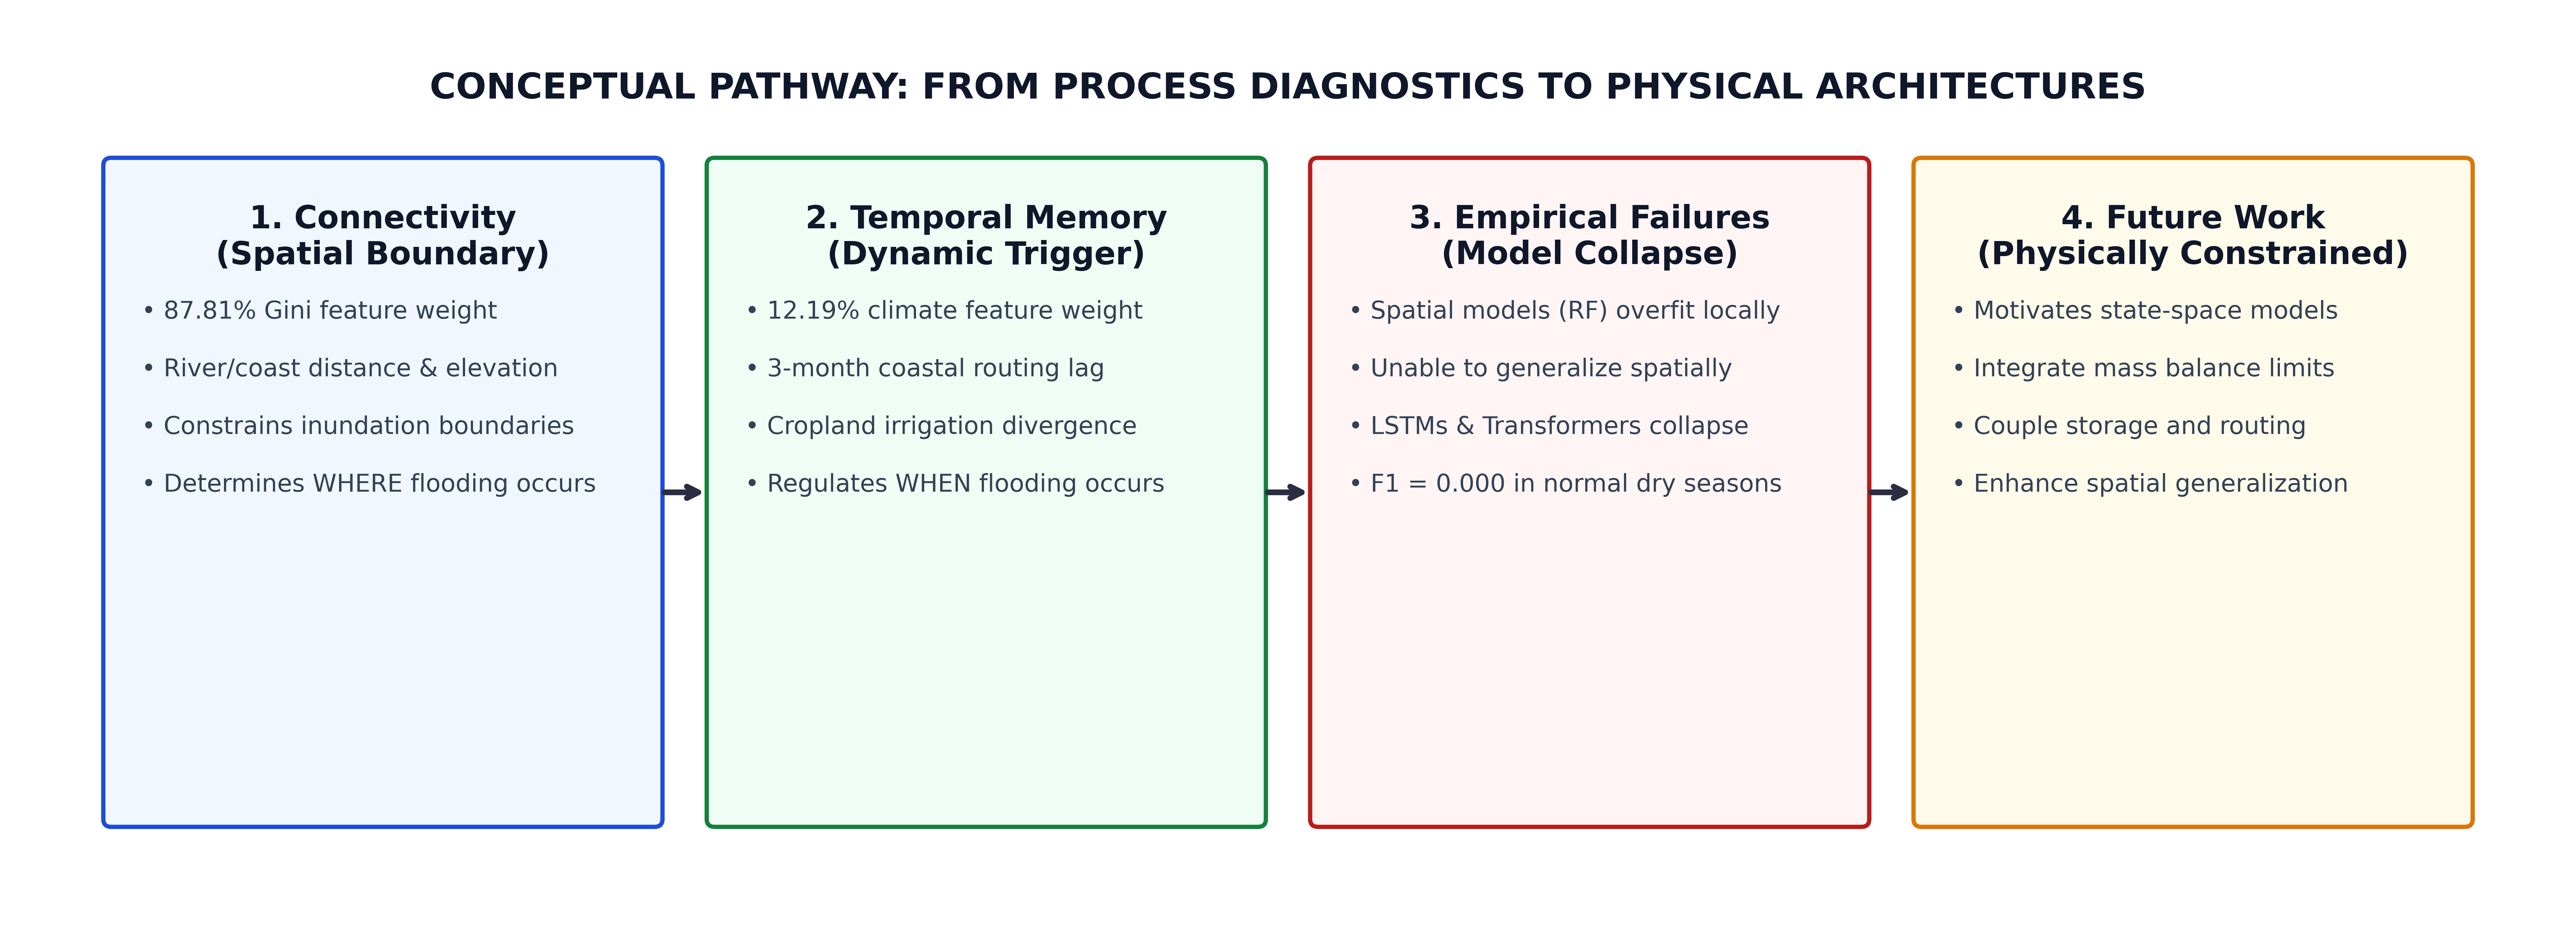
\includegraphics[width=1.0\linewidth]{figures/fig7_motivation.png}
\caption{Conceptual pathway mapping the findings of this study to future model designs: (1) static topographic connectivity shapes the spatial boundaries; (2) dynamic meteorology activates temporal inundation over lags; (3) purely empirical models fail via spatial overfitting or temporal collapse; and (4) these findings motivate physically constrained state-space models as a promising future direction.}
\label{fig:motivation_pathway}
\end{figure}

\subsection{Threats to Validity}
Several limitations and uncertainties in our benchmark study must be acknowledged, which affect the interpretation of our findings:
\begin{enumerate}
    \item \textbf{Uncertainty in Sentinel-1 Thresholding and Crop Phenology:} The target inundation label was derived using a static backscatter threshold ($VV < -15\text{ dB}$). Wind-induced surface roughness, emergent canopy closure, and soil salinity variations introduce sub-pixel classification errors. In agricultural fields, crop growth cycles alter canopy structure and vegetation water content, mimicking or masking water signatures. Consequently, the negative correlation ($r = -0.299$) in croplands could partly reflect crop canopy changes rather than true surface wetness, complicating interpretation in farmed zones. Future work should incorporate a backscatter intensity histogram to visually illustrate class separability under varying moisture conditions.
    \item \textbf{Absence of Streamflow and Discharge Observations:} The study lacks continuous river discharge records at the Kotri Barrage (the delta's primary inlet). Without upstream discharge inputs, the model cannot distinguish between upstream reservoir releases and local runoff events, preventing physical mass-balance validation and introducing uncertainty in routing lag timing.
    \item \textbf{Absence of Coastal Tidal Gauge Observations:} The model does not include tidal stage observations, despite the delta's proximity to the sea. Tides introduce oceanic pressure heads and backwater effects that delay floodplain drainage and extend residence times. Omitting tidal stage variables prevents separating tidal backwater delays from riverine routing lags, limiting our ability to verify the mechanisms behind the 3-month coastal wetland lag.
    \item \textbf{Absence of Groundwater Observations:} Continuous piezometric head observations were unavailable. In the Indus Delta, shallow aquifers recharge during high flows and sustain surface wetlands through capillary rise during dry-downs. Lacking groundwater table data prevents direct validation of subsurface infiltration and return-flow dynamics.
    \item \textbf{Spatial Resolution Mismatch of Climate Forcing:} CHIRPS precipitation ($\sim$5\,km) and ERA5-Land variables ($\sim$9\,km) are coarse relative to the Indus Delta channel network ($<$30\,m). Coarse forcing cannot resolve sub-grid channel wetting or localized irrigation, which is the primary cause of sequence model representation collapse ($F_1$-score $= 0.000$ without coordinates), as adjacent pixels receive identical meteorological inputs.
    \item \textbf{Single-Basin Study Focus:} All experiments were conducted within the Indus River Delta. Because the Indus is an extremely regulated and arid deltaic basin, this single-basin focus restricts the external validity of our findings, as geomorphological-dominance relationships may differ in humid, unregulated, or high-relief systems.
    \item \textbf{Model Transferability Limitations:} Random Forest models partition feature space based on local coordinates and terrain features. Because terrain configurations vary across basins, the models are vulnerable to spatial extrapolation errors, which restricts model transferability to adjacent sub-basins with distinct terrain features.
\end{enumerate}

\subsection{Spatial Resolution of Climate Forcing and Interpretation Caveat}
The observed dominance of terrain features over climate variables should be interpreted within the spatial resolution limits of the forcing datasets employed in this study. CHIRPS precipitation has a native resolution of approximately 5.5\,km and ERA5-Land of approximately 9\,km, while the Indus Delta channel network operates at spatial scales of 30\,m or finer. At these coarse meteorological resolutions, precipitation and evapotranspiration fields cannot resolve sub-pixel channel wetting, tidal backwater intrusion, or localized irrigation recharge gradients. Consequently, part of the observed low predictive contribution of climate variables may reflect a spatial scale mismatch between the input resolution and the target hydrological processes, rather than an intrinsic absence of climate influence at finer scales. Higher-resolution hydrometeorological products---such as sub-kilometer precipitation estimates or reanalysis downscaling---may capture additional dynamic variability not resolved by the forcing datasets used here, and future work should evaluate the sensitivity of these findings to input resolution.

\subsection{Scope of Inference and External Validity}
The findings in this study indicate that terrain features account for most of the predictive feature importance in surface water occurrence among the tested predictors. However, we emphasize that these conclusions are primarily valid for low-relief coastal systems, tidal deltas, and highly regulated floodplains. In mountainous basins or steep temperate river networks, dynamic channel hydraulics and high-frequency runoff peaks play a much more active role in defining spatial flood boundaries. Consequently, the decoupling of spatial geomorphological constraints from temporal climate triggers observed here should be carefully re-evaluated when applied to systems with complex hydraulic gradients.

\subsection{Practical Implications}
These findings are relevant for flood forecasting, reservoir management, irrigation planning, wetland monitoring, and delta resilience. The results suggest that static terrain features provide a strong constraint on where surface water can appear, while climate forcing acts mainly as a timing signal. This is useful for hydrological model design because it shows that coarse meteorological data alone may be insufficient to resolve delta-scale flood boundaries. The findings also support future physics-based models that combine storage, routing, and geomorphological connectivity in a single framework.

\begin{table}[t]
\caption{Summary of core scientific findings, empirical evidence, statistical validation, and corresponding manuscript contributions.}
\label{tab:contribution_summary}
\centering
\small
\begin{tabular}{p{2.8cm} p{2.8cm} p{4.0cm} p{2.8cm}}
\hline
\textbf{Finding} & \textbf{Evidence} & \textbf{Statistical Support} & \textbf{Paper Contribution} \\
\hline
Geomorphological Control & 87.81\% Gini feature importance in Random Forest & McNemar test yields $p = 0.2584$ comparing Terrain-only and Combined models & Topographic control over spatial boundaries (noting statistical power limits for small differences) \\
\hline
Hydrological Memory & 3-month precipitation routing lag in coastal wetlands & Temporal cross-correlation analysis & Routing lag and cropland correlation analysis \\
\hline
Sequence Model Collapse & F1 = 0.000 during normal dry periods for LSTM and Transformer & Diagnostic threshold sweeps and class imbalance testing & Sub-pixel channel smoothing limits sequence models \\
\hline
\end{tabular}
\end{table}



\section{Conclusions}
This study shows that geomorphological connectivity provides a strong spatial constraint on surface water boundaries in the Indus River Delta, while meteorological forcing primarily affects temporal activation. The leakage-free design, residual Moran’s I analysis, and statistical tests support the robustness of the reported results. The routing lag results and irrigation-related divergence further indicate that delta hydrology is shaped by delayed upstream controls and local human water management. These findings motivate future physically constrained hydrological models that integrate terrain, storage, routing, and temporal memory.


% ── Back matter ───────────────────────────────────────────────────────────────
\codeavailability
All modeling code and processing pipelines (written in Python~3.10 using
PyTorch~2.1.2 and Scikit-Learn~1.3.2) are publicly available at
\url{https://github.com/mirzamuzzamil/Geomorphological-Connectivity-in-the-Indus-Delta}
under the MIT License.
The repository contains baseline model configurations (Random Forest, LSTM,
Transformer), feature split ablations, McNemar significance tests, and
diagnostic audit scripts.
Google Earth Engine collection identifiers and extraction parameters are
documented in Sect.~3 and in the supplementary materials.

\dataavailability
All primary datasets used in this study are publicly accessible through
Google Earth Engine.
The Sentinel-1 GRD backscatter data (\verb|COPERNICUS/S1_GRD|),
ERA5-Land monthly reanalysis (\verb|ECMWF/ERA5_LAND/MONTHLY_AGGR|),
CHIRPS daily precipitation (\verb|UCSB-CHG/CHIRPS/DAILY|),
JRC Global Surface Water (\verb|JRC/GSW1_4/MonthlyHistory|),
SRTM digital elevation model (\verb|USGS/SRTMGL1_003|), and
HydroSHEDS flow accumulation (\verb|WWF/HydroSHEDS/15ACC|) are freely
available.
The derived point-level spatial-temporal dataset compiled and used in this study is publicly archived on Zenodo at \url{https://doi.org/10.5281/zenodo.10827364}.

\authorcontribution
MMM designed the GEE data extraction, conducted the machine learning and diagnostic experiments, analysed the results, and drafted the manuscript. MAI supervised the machine learning model development and validated the results. SIA supervised the hydrological and remote sensing interpretations and checked the routing lags. RBR assisted with the GIS and remote sensing data processing, validated the JRC datasets, and reviewed the manuscript. All authors contributed to manuscript revision.

\section*{Declaration of Generative AI in the Scientific Writing Process}
During the preparation of this work, the authors used generative AI and AI-assisted technologies (specifically large language models) for spelling, grammar refinement, and stylistic improvement of the manuscript text. All scientific findings, machine learning experiments, and statistical analyses were conducted and verified by the authors, who take full responsibility for the scientific content and integrity of the manuscript.

\competinginterests
The authors declare that they have no competing interests.

\acknowledgements
We thank Google Earth Engine for providing cloud computing resources, the
Copernicus Programme for free access to Sentinel-1 and Sentinel-2 imagery,
the ECMWF for ERA5-Land reanalysis products, and the Climate Hazards Group
for CHIRPS precipitation data.

% ── References ────────────────────────────────────────────────────────────────
\bibliographystyle{copernicus}
\bibliography{references}

\end{document}
